
%%%%%%%%%%%%%%%%%%%%%%%%%%%%%%%%%%%%%%%%%
% Short Sectioned Assignment
% LaTeX Template
% Version 1.0 (5/5/12)
%
% This template has been downloaded from:
% http://www.LaTeXTemplates.com
%
% Original author:
% Frits Wenneker (http://www.howtotex.com)
%
% License:
% CC BY-NC-SA 3.0 (http://creativecommons.org/licenses/by-nc-sa/3.0/)
%
%%%%%%%%%%%%%%%%%%%%%%%%%%%%%%%%%%%%%%%%%

%----------------------------------------------------------------------------------------
%	PACKAGES AND OTHER DOCUMENT CONFIGURATIONS
%----------------------------------------------------------------------------------------

\documentclass[paper=a4, fontsize=11pt]{scrartcl} % A4 paper and 11pt font size

\usepackage[T1]{fontenc} % Use 8-bit encoding that has 256 glyphs
\usepackage{fourier} % Use the Adobe Utopia font for the document - comment this line to return to the LaTeX default
\usepackage[english]{babel} % English language/hyphenation
\usepackage{amsmath,amsfonts,amsthm} % Math packages
\usepackage{bm}
\usepackage{mathtools}
\usepackage{graphicx}
\usepackage{amsmath}
\DeclareMathOperator*{\argmax}{arg\,max}
\DeclareMathOperator*{\argmin}{arg\,min}

\usepackage{sectsty} % Allows customizing section commands
\usepackage{hyperref} % URL package
\usepackage[title]{appendix}


\usepackage{listings}
\usepackage[utf8]{inputenc}

\usepackage{listings}
\usepackage{color}
\usepackage{tikz}
\usepackage{grffile}

\usetikzlibrary{positioning}

\definecolor{codegreen}{rgb}{0,0.6,0}
\definecolor{codegray}{rgb}{0.5,0.5,0.5}
\definecolor{codepurple}{rgb}{0.58,0,0.82}
\definecolor{backcolour}{rgb}{0.95,0.95,0.92}

\lstdefinestyle{mystyle}{
	backgroundcolor=\color{backcolour},   
	commentstyle=\color{codegreen},
	keywordstyle=\color{magenta},
	numberstyle=\tiny\color{codegray},
	stringstyle=\color{codepurple},
	basicstyle=\footnotesize,
	breakatwhitespace=false,         
	breaklines=true,                 
	captionpos=b,                    
	keepspaces=true,                 
	numbers=left,                    
	numbersep=5pt,                  
	showspaces=false,                
	showstringspaces=false,
	showtabs=false,                  
	tabsize=2
}

\lstset{style=mystyle}

\hypersetup{colorlinks,urlcolor=blue}
\allsectionsfont{\centering \normalfont\scshape} % Make all sections centered, the default font and small caps

\usepackage{fancyhdr} % Custom headers and footers
\pagestyle{fancyplain} % Makes all pages in the document conform to the custom headers and footers
\fancyhead{} % No page header - if you want one, create it in the same way as the footers below
\fancyfoot[L]{Vijaykumar} % Empty left footer
\fancyfoot[C]{} % Empty center footer
\fancyfoot[R]{\thepage} % Page numbering for right footer
\renewcommand{\headrulewidth}{0pt} % Remove header underlines
\renewcommand{\footrulewidth}{0pt} % Remove footer underlines
\setlength{\headheight}{13.6pt} % Customize the height of the header

%\numberwithin{equation}{section} % Number equations within sections (i.e. 1.1, 1.2, 2.1, 2.2 instead of 1, 2, 3, 4)
%\numberwithin{figure}{section} % Number figures within sections (i.e. 1.1, 1.2, 2.1, 2.2 instead of 1, 2, 3, 4)
%\numberwithin{table}{section} % Number tables within sections (i.e. 1.1, 1.2, 2.1, 2.2 instead of 1, 2, 3, 4)

\setlength\parindent{0pt} % Removes all indentation from paragraphs - comment this line for an assignment with lots of text

\usepackage{graphicx}
\usepackage{grffile}
\usepackage[justification=centering]{caption}
\usepackage{subcaption}
\usepackage{float}
%\usepackage{subfigure}
\usepackage{subcaption}
\usepackage{multirow}

\usepackage[ruled,vlined]{algorithm2e}

\usepackage{fancyvrb}

\newcommand{\be}{\begin{equation}}
\newcommand{\ee}{\end{equation}}

% redefine \VerbatimInput
\RecustomVerbatimCommand{\VerbatimInput}{VerbatimInput}%
{fontsize=\footnotesize,
	%
	frame=lines,  % top and bottom rule only
	framesep=2em, % separation between frame and text
	rulecolor=\color{Gray},
	%
	label=\fbox{\color{Black}data.txt},
	labelposition=topline,
	%
	commandchars=\|\(\), % escape character and argument delimiters for
	% commands within the verbatim
	commentchar=*        % comment character
}

%----------------------------------------------------------------------------------------
%	TITLE SECTION
%----------------------------------------------------------------------------------------

\newcommand{\horrule}[1]{\rule{\linewidth}{#1}} % Create horizontal rule command with 1 argument of height

\title{	
\normalfont \normalsize 
\horrule{0.5pt} \\[0.4cm] % Thin top horizontal rule
\LARGE CSCE 636 Deep Learning \\
\LARGE Assignment1 Report \\ % The home/pbehne/git\_repos/CSCE633\_S20\_PATRICK\_BEHNE/hw1/dataset/assignment title
\horrule{2pt} \\[0.5cm] % Thick bottom horizontal rule
}

\author{Akhilesh Vijaykumar} % Your name
\begin{document}

\maketitle % Print the title

%----------------------------------------------------------------------------------------
\begin{enumerate}
	\item \begin{enumerate}
		\item Two
		\item Three
		\item Four
	\end{enumerate}
	\item Five
	\item Six
\end{enumerate}

\section{Introduction} \label{sec: intro}

The goal of this project is to employ and optimize different machine learning algorithms to solve a classification problem.
The data-set for this classification problem contains information (features) that describes the execution of different programs.
These programs can take one of two classifications: benign or malicious.
In addition to the methods investigated in previous assignments (decision trees, perceptrons, ensemble learners, and $k$ nearest neighbors), this project will additionally explore the application of neural networks to this problem.
\\

The primary focus of this assignment will be the application of neural networks to this problem and optimization strategies of each of the methods.
For brevity, outlines of the algorithms previously used in other assignments are omitted.
If necessary, the algorithm descriptions can be found in Zach and Patrick's homework two report and Zach, Patrick, Hanzhou, and Jiacong's homework three report.
Different types of optimizations will be discussed throughout the report, including input transformation effects, parameter tuning, and feature selection.
\\


The remainder of this report is as follows.
Section \ref{sec: software} presents the necessary software to execute the programs.
Section \ref{sec: structure} describes the organization of the source code and the general flow of the programs.
Section \ref{sec: features} presents the methodology used to select optimal features for model inputs.
Following this, Section \ref{sec: input scaling} discusses the different options available to scale the raw feature values.
Sections \ref{sec: neural net} and \ref{sec: novel} present the algorithms, optimizations and results from a neural network and the novel learner, respectively.
The novel learner from Section \ref{sec: novel} is then compared to all other models in Section \ref{sec: compare}.
Finally, concluding remarks are made in Section \ref{sec: conclusion}.
	
\section{Software Requirements} \label{sec: software}

Because the data-set is relatively small and there is plentiful open source software available, the high-level object-oriented programming language Python is used in this assignment.
The open source software heavily utilized throughout this assignment are Pandas, a data analysis package, Scikit-Learn, a machine-learning package, Graphviz, a visualization package, prettytable, a table package, and progressbar2, a status package. 
The latter three of these packages often is not standard with a Python distribution and can be installed via pip or conda, whichever is appropriate for the system. 
Graphviz package is used only for displaying nice decision trees, so if desired, one can comment out any commands using this package and forego the installation.
The prior packages generally come standard in Python distributions and can be installed similarly if necessary.

\section{Program Structure} \label{sec: structure}

This section discusses the organization of the source code directory and goes into detail on the construction, strategy, and flow of the source code.

\subsection*{Organization of Source Code}

The {\em src} directory is organized into several different sub-directories.
In the root of {\em src} lies the driver class \verb|Project|, which ultimately initializes, trains, and evaluates the different machine learning models.
This directory also contains all of the run files required to produce any results seen in this report.
The {\em learners} sub-directory contains all of the modules for each of the machine learning models.
These are discussed in detail in the following subsection.
The {\em studies} sub-directory contains files containing different methods used to exercise the different learning models.
Lastly, the {\em utilities} sub-directory contains auxiliary routines such as parsing and preparing data.

\subsection*{Data Preparation}

The data preparation is handled off-line using the \verb|DataPreparation| class.
This class parses the program data-sets for a specified list of features and programs.
The inputs to initialize this class are the root directory of the data-set, the file name within the root directory containing the feature names, and the file name within the root directory containing the program names.
A check is performed to filter out duplicate features and programs.
A series of checks is performed to ensure no duplicate items are parsed and that no issues arise when searching for files.
For features, this just requires filtering for duplicates.
For programs, a bit more attention must be paid.
Programs are specified as either the base name of a program or the base name with a snapshot identifier appended to it.
Regardless the input, the program names specified are stripped to their base names and then a check for duplicates ensues.
After this a secondary program names list is compiled by iterating through the program directories of the data-set.
For each program directory in the data-set, if its base name matches one of those within the list of unique program base names and the directory contains a {\em stats.txt} file, the specific program snapshot is added to the list of those to parse.
\\

The parsing routine simply builds up a Pandas DataFrame by sequentially adding dictionaries of features and their respective values for each program.
After the parsing is complete, any missing values are filled with the specified value.
Following this, features values are checked for variance.
If a feature value is constant across all programs, it is removed from the data-set because it can provide no information.
As a last step, the data is normalized if specified by the user.
Routines exist to normalize the data in five ways: 1) to the maximum value of each feature, 2) to the global maximum, 3) to the mean value of each feature, 4) to the global mean value, and 5) subtracting the mean of each feature and dividing by that feature's standard deviation.

\subsection*{Learning Models}

The different learning models are all derived from a base class, \verb|LearnerBase|, which is in turn derived from the \verb|BaseEstimator| and \verb|ClassifierMixin| classes, which are skeleton Scikit-Learn estimator interfaces \cite{scikit-learn}.
\verb|LearnerBase| has one default member, \verb|learner_|, and four default functions, \verb|fit|, \verb|score|, \verb|predict|, and \verb|set_params|.
The \verb|learner_| attribute is set to a Scikit-Learn estimator in the derived class, and the default \verb|fit|, \verb|score|, and \verb|predict| methods simply call the Scikit-Learn estimator, \verb|learner_|'s \verb|fit|, \verb|score|, and \verb|predict| functions.
The derived class must implement the \verb|fit|, \verb|score|, and \verb|predict| methods if these methods are not simply a call to a Scikit-Learn method.
The \verb|set_params| method is useful when using Scikit-Learn's \verb|GridSearchCV| function to discover hyper-parameters.
By constructing the learners in a consistent way, many of the same routines may be recycled making the addition of new learning models is quite simple.
The following sub-section will expand upon this.
\\

\subsection*{Model Evaluations}

Model evaluations are streamlined through the \verb|Project| class.
This class is initialized with inputs of the data, the model type, and a corresponding set of hyper-parameters defined by the author of the model selected, and other information such as the number of folds in the cross-validation suite and the level of statistical confidence desired.
At initialization, this class initializes the specified learner with the given hyper-parameters and stores the other inputs.
\\

Models are evaluated using the \verb|evaluate_model_accuracy| method.
First the routine splits the data using Scikit-Learn's \verb|StratifiedKFold| into $K$ training and test sets.
The ``Stratified'' variant of this class is used because it preserves the fraction of different classification types in the full data-set within each of the training and test sets.
This is useful because it helps reduce the effects that shuffling may have on the performance of a model.
If the data-set is very small, this effect can be profound.
Next, the method iterates through each of the folds, training the model on the prescribed training set and then testing it with the reserved test set.
Through the cross-validation suite, accuracy, variance, and training and test times are kept.
Additionally, the best model is stored throughout.
The output of this function is all relevant information describing the model performance.

\section{Input Transformations} \label{sec: input scaling}
\subsection*{Shifting and Normalizations}
This section will discuss the different input transformations applied to the data-set to aid in increasing performance of each of the learning models.
In many cases, the normalization or standardization of a data-set can influence the performance of a learning model.
Five general input transformations are available: 
\begin{enumerate}
	\item Dividing by the maximum value, 
	\item Mapping to a specified interval, 
	\item Dividing by the $\ell^2$-norm of the feature vector, 
	\item Removing the mean value and dividing by the standard deviation, and 
	\item Removing the median and dividing by the inter-quartile range.
\end{enumerate}
Not all are discussed in this report, however, all are available to the user.
\\
These transformations are applied differently than in the previous two assignments.
Before, the full data-set was normalized by considering observed values over all samples.
This was performed before the the data were split into cross-validation folds and training and test sets.
By doing this, it is possible that some bias is introduced into the results.
Take, for instance, a data-set which has outliers that are dramatically different from the average value across the data-set.
If the full data-set is considered in the normalization, these samples can influence the normalization significantly.
In this work, raw data are transformed in each cross-validation fold by considering only the training data.
The test data is then transformed by identically to the training data.
For instance, with maximum value normalization, the test data is normalized to the maximum observed value over the training set.
By doing this, the test data is truly unseen by the model before testing.
\\
Normalization by maximum values is a simple technique that, maps the value of each input to a magnitude less than unity.
This normalization can lead to better performance in models because it removes any intrinsic influence features of significantly larger magnitude may have on the model.
There are no requirements on the underlying data-set to use this normalization.
This normalization is particularly susceptible to the influence of large values outliers.
Mapping to a specified interval and dividing by the norm of the feature have very similar effects and requirements.
\\
Removing the mean and dividing by the standard deviation implicitly makes the assumption that the data approximately follows a normal distribution and has non-zero variance.
If this is the case, the result of this normalization is a data-set with a zero mean and unit standard deviation.
This technique is often used because the effects of outlier data are significantly diminished.
Further, with this normalization, an input signal is proportional to its likelihood.
This is favorable for models which learn relative to the size of the inputs because those instances which do not often occur receive more weight.
If a data-set has many outliers such that the mean and standard deviation are influenced in a non-negligible way, this normalization will be less well behaved.
\\
The alternative to the above normalization is removing the median and dividing by the inter-quartile range.
The inter-quartile range is defined to be the difference in the median of upper half of the data and the median of the lower half of the data.
This normalization reduces the influence of outlier data even more than the above technique by using median values instead of means.
The properties of this resultant data-set, while similar to the previous normalization, are somewhat less nice.
\\
Within each of these normalization methods, two strategies are employed: 1) Normalization across the full data-set, and 2) normalization across samples with the same time stamp.
The prior is self explanatory so only the latter is discussed here.
Within the data-set, many of the samples are of the same program, but at a different time slice.
To do this, a routine was implemented that identifies the unique time slices, groups samples by these time slices, and performs either of the aforementioned normalization methods on these subsets.
The logic behind this normalization is to account for features which scale with time across all programs, such as committed instructions.
If the maximum value for a feature that scales with time is used for normalization, then the programs at early time slices have little contribution to the activation of any given neuron.
The implementation of these methods use various of Scikit-Learn's \verb|preprocessing| modules \cite{scikit-learn}.
\\
\subsection*{Principal Component Analysis}
Principal component analysis (PCA) is a dimensionality reduction technique.
This technique uses the singular value decomposition (SVD) to project high-dimensional data onto a low-dimensional, orthogonal coordinate system.
First, one centers the data by removing the mean from the data-set column-wise.
Consider the shifted data-set $B = X - \bar{X}$, which is an $M \times N$ matrix.
The singular value decomposition of $B$ gives $B = U \Sigma V^T$.
$U$ is a unitary, $M \times M$ matrix containing the eigenvectors of $B B^T$.
$\Sigma$ is a diagonal $M \times N$ matrix containing the singular values of $B$, given by the square root of the eigenvalues of $B^T B$.
$V$ is a unitary, $N \times N$ matrix containing the eigenvectors of $B^T B$.
The dimensionality reduction occurs by truncating the SVD matrices along the inner dimensions of the product $U \Sigma V^T$.
If $K$ components are desired, this product then becomes the product of an $M \times K$, $K \times K$, and $K \times N$.
The principal component coordinates of the data-set are then given by a projection of the data-set onto the eigenvectors of the covariance matrix (principal components), $V$, such that $T = B V = U \Sigma$.
With this, the data-set is comprised of $K \ll N $ orthogonal, and therefore uncorrelated, features for each of the $M$ samples.
\\
In practice, these components are ordered based upon the magnitude of its corresponding singular value.
The amount of explained variance contained within a component is given by the square of the singular value for that component divided by the total sum of squares of all singular values.
There are two general ways to specify a truncation:
\begin{enumerate}
	\item An integer number of components to keep.
	\item A cutoff for the fraction of the explained variance to keep.
\end{enumerate}
The prior is self explanatory.
The latter keeps the components (ordered most informative to least) whose relative explained variance sums to the threshold value, truncating all further modes.
The relative error in this truncation procedure is proportional to the relative explained variance truncated.
For example, Figure \ref{fig: decomposition} shows the decay of the singular values from the data-set.
The implementation of this was carried out using Scikit-Learn's \verb|PCA| class.
It should be noted that as with the normalization methods, PCA is applied only to training sets such that bias is not introduced to the model \cite{scikit-learn} \cite{pcaWiki} \cite{pcaTDS}. 
\begin{figure}[H]
	\centering
	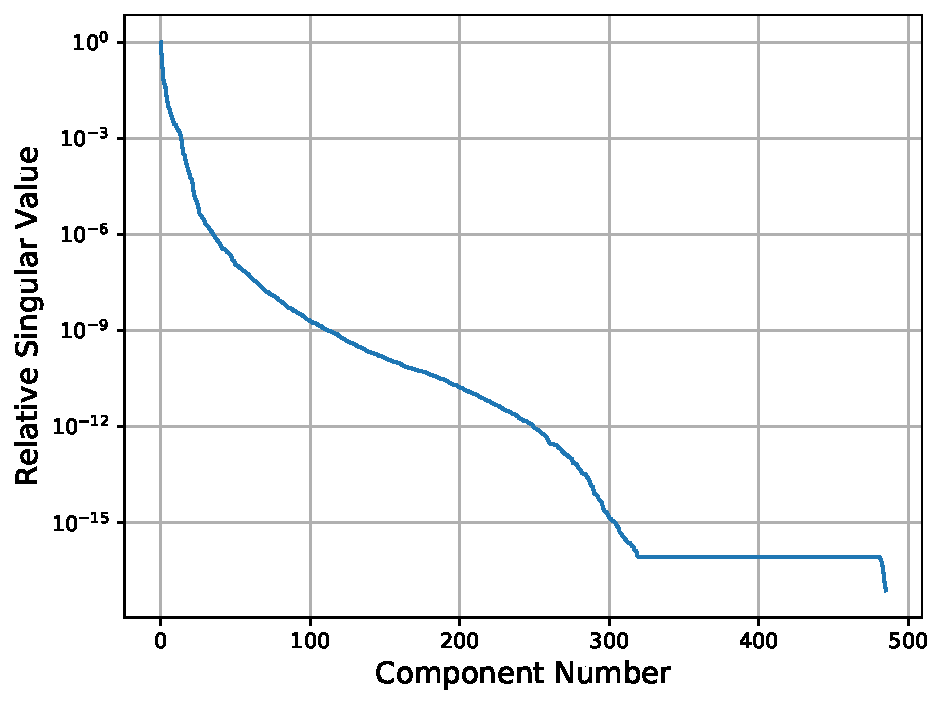
\includegraphics[scale=0.6]{figures/pca.pdf}
	\caption{Singular value decay for the data-set.}
	\label{fig: decomposition}
\end{figure}


\section{Feature Selection} \label{sec: features}

This section discusses the strategies used to filter out noise from the data-set and select only features that are distinct and informative of a program's classification.

\subsection*{Correlation Between Features}

In this work we investigate two metrics to measure the similarity between two features.
The first is adopted from linear algebra. 
Given two vectors, $x_i$ and $x_j$, containing the values for each program sample for feature $i$ and $j$, we define the following measure for the  correlation between them:
\begin{equation}
\small
c_{i,j}=\frac{x_i \cdot x_j}{||x_i||||x_j||},
\end{equation}
which is equivalent to the cosine of the angle between the two vectors.
This number is in the [-1,1] interval. 
The values of $\pm$1 indicate that the two vectors are the same or completely opposite, while a value of 0 means that the two vectors are orthogonal.
It is important to mention that the dot product function \texttt{np.dot()} of \texttt{numpy} can be slow for large data vectors depending on what BLAS (linear algebra package) is installed on the system.
If the user experiences slow operation with this correlation definition, one is recommended to switch to the following correlation metric.  

The Pearson correlation \cite{murphy2012machine} can be defined as follows (with the same notation):
\begin{equation}
\small
c_{i,j} = \frac{\sum\limits_{k=1}^{N} (x_{i,k} - \bar{x}_i)(x_{j,k} - \bar{x}_j)}
{\sqrt{\sum\limits_{k=1}^{N} (x_{i,k} - \bar{x}_i)^2 \sum\limits_{k=1}^{N} (x_{j,k} - \bar{x}_j)^2}}
\end{equation}
where $N$ denotes the number of program samples. 
The formula is derived by normalizing the covariance of the two data vectors using the product of their standard deviations.
These coefficients take on values between -1 and 1 indicating the extent to which the two variables are linearly related. 
A correlation of 0 indicates that two variables do not have a linear relationship.
It should be noted that a nonlinear relationship may still exist in this case.

A correlation filter algorithm is implemented to remove the discovered redundant (correlated) features.
The flow chart of the algorithm is presented in Figure \ref{fig:corr_filter}.

\begin{figure}[H]
	\centering
	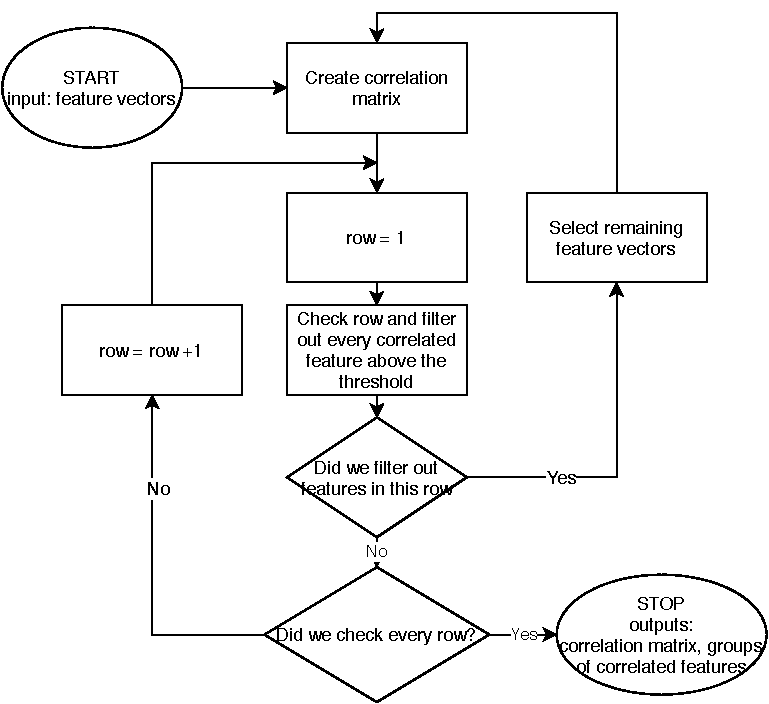
\includegraphics[width=0.5\linewidth]{figures/correlation_filter}
	\caption{The flow diagram of the correlation filter implemented in this homework.}
	\label{fig:corr_filter}
\end{figure}


It is assumed that feature $i$ and $j$ are closely correlated if their corresponding $|c_{i,j}|$ is above a user-defined threshold.
A correlation matrix is generated and based on the values of its entries, features are grouped together based on similarity.
From each of these groups, only a single feature is kept. 

After this filtering process, the feature groups are printed to the file
\begin{lstlisting}[language=python]
output/features/correlated_feature_groups*.txt
\end{lstlisting} 
This file contains one group in each row with the features separated using a single space.
The number of feature groups as a function of the similarity threshold is seen in Figure \ref{fig:feature-correlation} for the unnormalized data.

\begin{figure}[H]
	\centering
	\begin{subfigure}{0.7\linewidth}
		\centering
		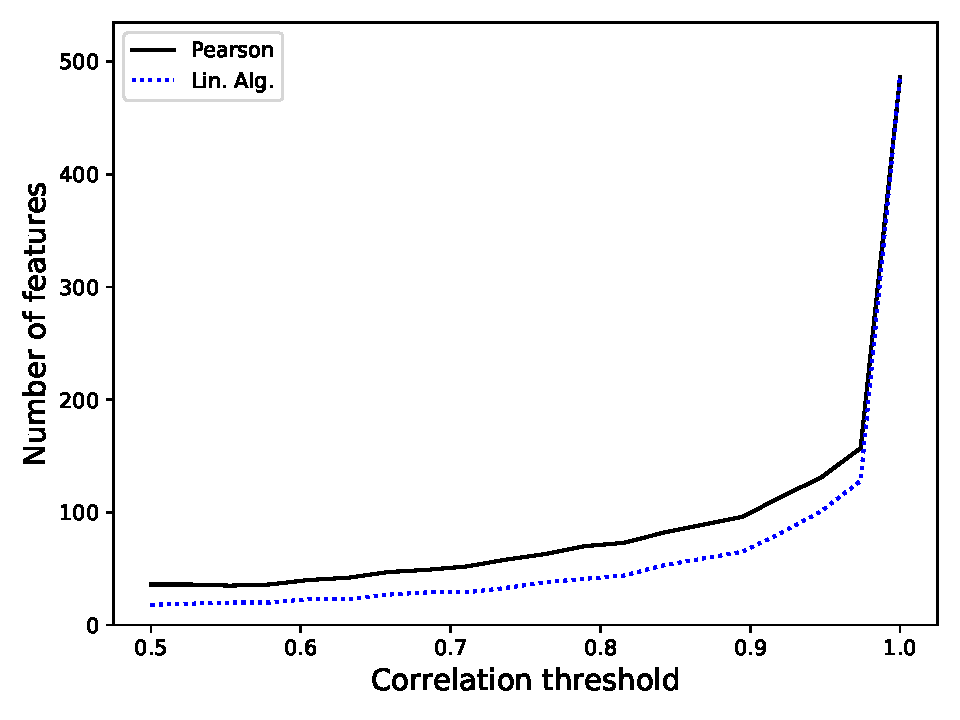
\includegraphics[width=1.0\linewidth]{../output/features/figures/global_max_feature_correlation}
	\end{subfigure}
	\caption{The number of features kept as function of the threshold of  the correlation filter.}
	\label{fig:feature-correlation}
\end{figure}

As expected, if the threshold is set to 1.0, all 486 features are retained.
A very small decrease in the threshold gives a dramatic decrease in the number of features.
It is also apparent that at a threshold of 0.7 only 40-50 features are kept with either correlation metric.
This suggests that many features in the data-set are redundant and by removing them, a considerable decrease in the training and classification cost can be achieved without compromising the information presented to the model.
It is interesting to note that the linear algebra correlation metric consistently removes more features with the same cut-off.

It must be also mentioned that the correlation between some of these features was exactly 1.0, implying that those features were exactly the same.
This provides some insight into the results from previous assignments.
Namely, this explains the seemingly fickle splitting in the root node of the decision tree model.
For a perceptron, using these redundant features would lead to the weight for a the single feature being split between all of the redundant occurrences of that feature, making any interpretation of weights as importance invalid.
For example with two identical attributes $x=x_1=x_2$ with $w_1$ and $w_2$ weights in the perceptron, assume that these weights can be summed into $(w_1+w_2)x$.

\subsection*{Feature-Label Correlation}

The same correlation coefficients can be computed using the feature vectors and the true label vectors ($y$) for each case: 
\begin{equation}
\small
c^y_{i}=\frac{x_i \cdot y}{||x_i||||y||}
\end{equation}
and
\begin{equation}
\small
c^y_{i} = \frac{\sum\limits_{k=1}^{N} (x_{i,k} - \bar{x}_i)(y_{k} - \bar{y})}
{\sqrt{\sum\limits_{k=1}^{N} (x_{i,k} - \bar{x}_i)^2 \sum\limits_{k=1}^{N} (y_{k} - \bar{y})^2}}.
\end{equation}

In this section, the correlation between the true label vector and the feature value vectors is investigated.
Both aforementioned correlation metrics are used for these evaluations.
The most correlated features from the 486 feature 941 sample data-set are summarized in Table~\ref{tab:corr_label_941_norm}.

It can be observed that 14 features of the top 20 are the same.
Even though the ranking of these features is not the same, the feature with the highest correlation to the label vector is \texttt{system.tol2bus.respLayer0.utilization} in both cases.
The label correlation filter implemented in this work slightly differs from the feature-feature correlation filter in terms of the definition of the cutoff threshold.
In this case, the threshold is given in the [0,1] interval and represents the fraction of the features that are kept.
For instance, 0.6 indicates that 60\% of the features most correlated to the label vector are kept. 

\begin{table}[H]
	\scriptsize
	\centering
	\caption{Most correlated features to the classification without any normlization on the data-set.}
	\label{tab:corr_label_941_norm}
	\begin{tabular}{|c|c|c|c|}
		\hline	
		Pearson & Value & Linear Algebra & Value \\
		\hline		
		system.tol2bus.respLayer0.utilization& 0.5741  & system.tol2bus.respLayer0.utilization& 0.7011 \\
		system.cpu.dcache.demand\_avg\_miss\_latency::total& 0.5473  & system.mem\_ctrls.bw\_inst\_read::total& 0.6899 \\
		system.cpu.dcache.overall\_avg\_miss\_latency::total& 0.5473  & system.cpu.icache.ReadReq\_mshr\_miss\_rate::total& 0.6861 \\
		system.mem\_ctrls.bw\_inst\_read::total& 0.5416  & system.cpu.icache.overall\_mshr\_miss\_rate::total& 0.6861 \\
		system.cpu.dcache.blocked\_cycles::no\_mshrs& 0.5308  & system.cpu.icache.demand\_mshr\_miss\_rate::total& 0.6861 \\
		system.cpu.icache.ReadReq\_mshr\_miss\_rate::total& 0.5091  & system.cpu.icache.ReadReq\_miss\_rate::total& 0.6817 \\
		system.cpu.icache.demand\_mshr\_miss\_rate::total& 0.5091  & system.cpu.icache.overall\_miss\_rate::total& 0.6817 \\
		system.cpu.icache.overall\_mshr\_miss\_rate::total& 0.5091  & system.cpu.icache.demand\_miss\_rate::total& 0.6817 \\
		system.mem\_ctrls.busUtil& 0.5074  & system.tol2bus.reqLayer0.utilization& 0.6462 \\
		system.mem\_ctrls\_0.averagePower& 0.5042  & system.mem\_ctrls.busUtil& 0.6419 \\
		system.cpu.icache.demand\_miss\_rate::total& 0.5001  & system.mem\_ctrls.bw\_total::total& 0.6382 \\
		system.cpu.icache.ReadReq\_miss\_rate::total& 0.5001  & system.mem\_ctrls.busUtilRead& 0.6363 \\
		system.cpu.icache.overall\_miss\_rate::total& 0.5001  & system.mem\_ctrls.avgRdBW& 0.6363 \\
		system.mem\_ctrls.bw\_total::total& 0.5000  & system.membus.respLayer1.utilization& 0.6325 \\
		system.cpu.dcache.ReadReq\_avg\_miss\_latency::total& 0.4938  & system.mem\_ctrls.avgRdBWSys& 0.6324 \\
		system.cpu.commit.op\_class\_0::FloatCvt& 0.4930  & system.mem\_ctrls.bw\_read::total& 0.6324 \\
		system.tol2bus.reqLayer0.utilization& 0.4903  & system.membus.reqLayer2.utilization& 0.6092 \\
		system.l2.ReadExReq\_mshr\_miss\_rate::total& 0.4851  & system.mem\_ctrls\_0.averagePower& 0.5906 \\
		system.l2.ReadExReq\_miss\_rate::total& 0.4851  & system.cpu.iq.fu\_busy\_rate& 0.5870 \\
		system.mem\_ctrls.busUtilRead& 0.4834  & system.cpu.dcache.ReadReq\_avg\_miss\_latency::total& 0.5821 \\	
		\hline
	\end{tabular}
\end{table}  

\section{Neural Network} \label{sec: neural net}

The following subsections describe the details of the training and test algorithms utilized for feed-forward neural networks and discuss the results obtained through various optimization experiments. 

\subsection*{Algorithm}
\label{sec:nn_algorithm}

Before discussing the details of the neural network itself, it is worth mentioning that in case of a binary classification problem, the \texttt{scikit-learn} objects perform an internal binary transformation on the input label vector. 
This consists of assigning a value of 1 to one class (malicious) and 0 to the other (benign) even if the input labels are within the {-1,1} set.
This enables the utilization of a cross-entropy loss function, discussed later in detail.  

A simplified drawing of a neural network with one hidden layer is presented in Figure \ref{fig:nn_drawing}.
Every edge corresponds to a weight and every neuron in the hidden and output layers contains a bias as well. 
At each node the outputs of the neurons in the preceding layer are summed up using the given weights and biases. 
To compute the output of a hidden node, an activation function is applied to this sum. 

\tikzset{%
	every neuron/.style={
		circle,
		draw,
		minimum size=1cm
	},
	neuron missing/.style={
		draw=none, 
		scale=4,
		text height=0.333cm,
		execute at begin node=\color{black}$\vdots$
	},
}

\begin{figure}[H]
	\centering
	\scalebox{0.65}{
	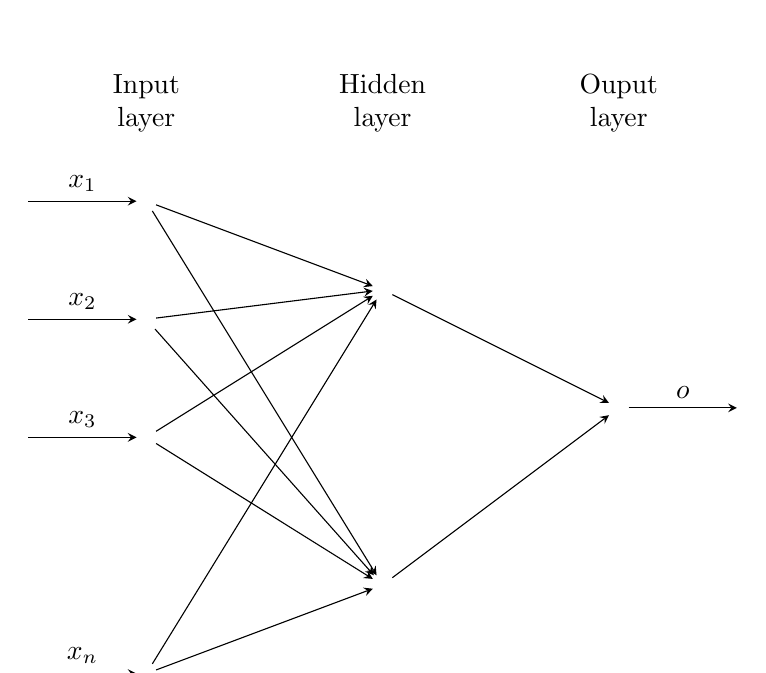
\begin{tikzpicture}[x=1.5cm, y=1.5cm, >=stealth]
		\foreach \m/\l [count=\y] in {1,2,3,missing,4}
		\node [every neuron/.try, neuron \m/.try] (input-\m) at (0,2.5-\y) {};
		
		\foreach \m [count=\y] in {1,missing,2}
		\node [every neuron/.try, neuron \m/.try ] (hidden-\m) at (2,2-\y*1.25) {};
		
		\foreach \m [count=\y] in {1}
		\node [every neuron/.try, neuron \m/.try ] (output-\m) at (4,0.75-\y) {};
		
		\foreach \l [count=\i] in {1,2,3,n}
		\draw [<-] (input-\i) -- ++(-1,0)
		node [above, midway] {$x_\l$};
		
		\foreach \l [count=\i] in {1}
		\draw [->] (output-\i) -- ++(1,0)
		node [above, midway] {$o$};
		
		\foreach \i in {1,...,4}
		\foreach \j in {1,...,2}
		\draw [->] (input-\i) -- (hidden-\j);
		
		\foreach \i in {1,...,2}
		\foreach \j in {1}
		\draw [->] (hidden-\i) -- (output-\j);
		
		\foreach \l [count=\x from 0] in {Input, Hidden, Ouput}
		\node [align=center, above] at (\x*2,2) {\l \\ layer};
		
	\end{tikzpicture}
	}
	\caption{The architecture of a typical neural network.}
	\label{fig:nn_drawing}
\end{figure}

Using this example, the nonlinear decision function 
\[ h(\textbf{x}) =  \left\{
\begin{array}{ll}
-1 & \text{if benign} \\
1 &  \text{if malicious} \\
\end{array} 
\right. \]
is approximated by 
\begin{equation}
\label{eq:nn_approx}
h(\textbf{x})\approx a^*\left(\sum\limits_{i=1}^{N_l}w_{o,i}a(\textbf{w}_{o-1,i}\textbf{x}+b_i)+b_o\right),
\end{equation}
where $a(x)$ and $a^*(x)$ are the activation functions in the hidden and output layers, respectively. 
Moreover, $w_{o,i}$ denotes the weight corresponding to the edge that connects the output node and the $i$-th neuron in the hidden layer.
$\textbf{x}=[x_1, x_2, ...]^T$ describes the input (feature) vector while $\textbf{w}_{o-1,i}$ is a vector of weights corresponding to the edges between the input neurons and the $i$-th neuron in the hidden layer.
Lastly, $b_i$ and $b_o$ are the biases in the corresponding neurons.
Of course, this notation can be generalized to deeper networks with more hidden layers by adding more nested activation functions connected with more weights and biases.

Depending on the problem at hand, different activation functions can be used in the neurons in the hidden layer. 
This work contains experiments with the following activation functions (see also Figure \ref{fig:act_functions}):
\begin{enumerate}
	\item $a(x) = tanh(x)=\frac{e^x-e^{-x}}{e^x+e^{-x}}$,
	\item $a(x) = \sigma(x)=\frac{e^{x}}{1+e^{x}}$, and
	\item $a(x) = relu(x)=\max(0, x)$
\end{enumerate}

where $ReLU$ stands for Rectified Linear Unit.
In the output layer, on the other hand, only a sigmoid function is used ($a^*(x)=\sigma(x)$) to make sure that the output is in the [0,1] domain.
This is also required for the cross-entropy loss function which is the default in \texttt{scikit-learn}.

\begin{figure}[H]
	\centering
	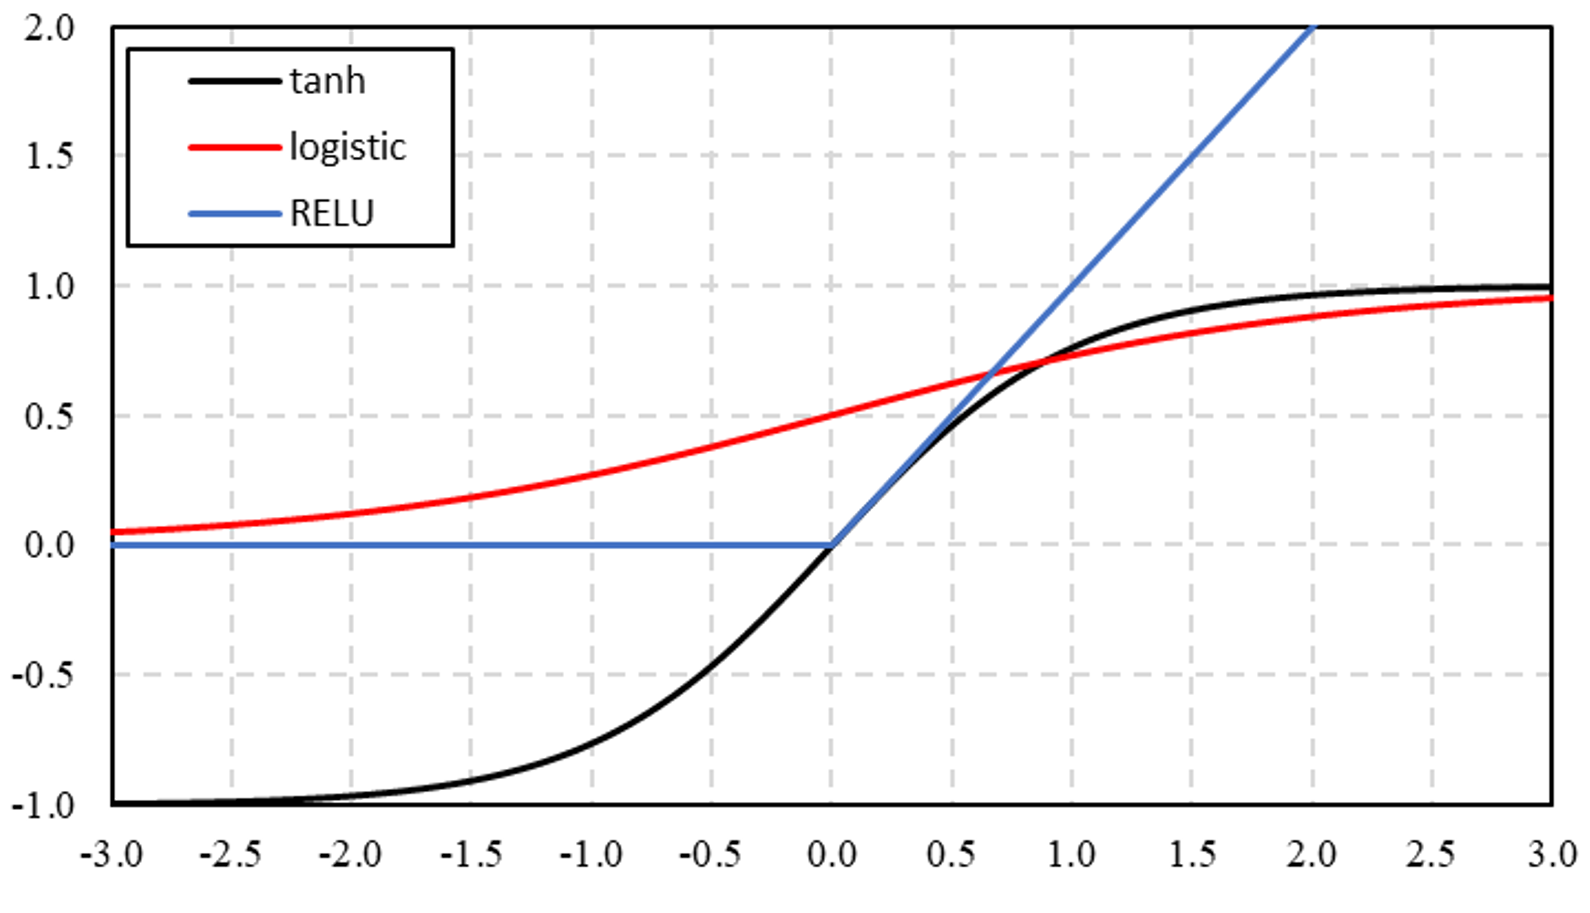
\includegraphics[width=0.55\linewidth]{figures/activation_function}
	\caption{Different activation functions used for the neurons.}
	\label{fig:act_functions}
\end{figure}

The model parameters in every case are the weights and biases in Eq. \eqref{eq:nn_approx}.
They can be determined using a stochastic gradient descent optimization with a binary cross-entropy loss function:
\begin{equation}
L(y,o,\textbf{W})=-y\text{ln}(o)-(1-y)\text{ln}(1-o)+\alpha ||\textbf{W}||_2^2,
\label{eq:loss}
\end{equation}
where $o$ is the output of the neural network and $y$ is the true class for the label after the binary transformation.
The advantages of this loss function over the regular squared difference loss function are summarized in \cite{Goodfellow-et-al-2016}.
Furthermore, to make sure that the weights of the neural network do not increase indefinitely, we apply an $L^2$ regularization by including a penalty term constructed using the magnitude of the weights in the loss function. 
This is described by $\alpha ||\textbf{W}||_2^2$ in Eq. \eqref{eq:loss} where the penalty factor $\alpha$ is a hyper parameter of the algorithm.

This loss function can be minimized using a gradient descent algorithm through back-propagation. 
The Adam (Adaptive moment estimation) algorithm \cite{kingma2014adam} is used in this work.
It is practically a stochastic gradient method, however it contains a moving average of the mean and uncentered variance of the gradient.
These increase the robustness and inherently add adaptivity to the method.
For more information the reader is referred to \cite{kingma2014adam}. 
This algorithm can be used for stochastic, mini-batch, and batch learning.

After the neural network is trained, an unknown sample can be evaluated by plugging in the new inputs in Eq. \eqref{eq:nn_approx} and applying the inverse of the binary transformation mentioned at the beginning of this section.
The inverse transformation maps the [0,1] interval onto the {-1,1} set by assigning -1 if the output is below 0.5 and 1 of it is above 0.5.

Lastly, a few terms for the stochastic gradient descend are defined for the sake of clarity and consistency:
\begin{enumerate}
	\item \textbf{Number of iterations:} describes how many times the weights are updated.
	\item \textbf{Number of epochs:} describes the number of times the iteration goes through the entire training data-set.
\end{enumerate} 
 
\subsection*{Model Complexity}

It is assumed that the neural network uses stochastic gradient descent, meaning that the weights and biases are updated after each sample.
Let $N$ denote the number of samples, $D$ the number of features, $L$ the number of hidden layers, and $H$ the number of perceptrons per layer. 
Furthermore, $I$ is used for the number of epochs needed to converge the model parameters and $O$ stands for the number of output neurons.
\noindent The \textbf{training phase} consists of two steps: 
\begin{enumerate}
	\item \textbf{Forward pass:}
	This involves the generation of scalar products with an overall complexity of $\mathcal{O}\left(D\cdot H + H^{L-1} + O\cdot H\right)$. 
	Assuming that all of the samples are used at least once, this becomes $\mathcal{O}\left(N\cdot \left[D\cdot H + H^{L-1} + O\cdot H\right]\right)$.
	Usually, multiple epochs are used in the stochastic gradient descend, so the prospective complexity grows to \\ $\mathcal{O}\left(I\cdot N\cdot \left[D\cdot H + H^{L-1} + O\cdot H\right]\right)$.
	\item \textbf{Backpropagation:}
	This phase involves the computation of the loss function which has a complexity of $\mathcal{O}(1)$ for one sample (with one output), but it grows to $\mathcal{O}(N)$ if all of the samples are used in the stochastic gradient descend and further increases to $\mathcal{O}(N\cdot I)$ if multiple epochs are needed.
	Updating the weights has a cost of $\mathcal{O}(D\cdot H+H^{L-1}+O \cdot H)$ for one update and $\mathcal{O}\left(N \cdot[D\cdot H+H^{L-1}+O \cdot H]\right)$ if a stochastic gradient descend is used with every sample.
	This also means that given $I$ iterations these all add up to $\mathcal{O}\left(I \cdot N \cdot[D\cdot H+H^{L-1}+O \cdot H]\right)$ again.
\end{enumerate}
So altogether these contributions add up to:
\\
\\
\textbf{Training time complexity:} $\mathcal{O}\left(I\cdot N\cdot [D\cdot H + H^{L-1} + O\cdot H]\right)$     
\\
\\ 
which is considerably higher than that of a single perceptron ($I\cdot N\cdot D$).
The classification of a new sample requires a forward pass only, meaning that the test time complexity is: 
\\
\\
\textbf{Test time complexity:} $\mathcal{O}\left(I\cdot N\cdot [D\cdot H + H^{L-1} + O\cdot H]\right)$
\\
\\
It must be emphasized that if a new sample is added to the training set the computational price to modify this learner is low, it requires a forward pass and a backpropagation sweep in an optimal case. 
In a pessimistic scenario, however, it may take multiple stochastic gradient steps to converge to new weights.
In terms of \textbf{memory usage}, the complexity of this method scales with the number of features, and hidden and output layers:
\\
\\
\textbf{Space complexity:} $\mathcal{O}(D\cdot H+H^{L-1}+O\cdot H)$
\\
\\
because the parameters can be updated after each iteration and storing old parameters is not necessary.

\subsection*{Optimizations}
In this work six different methods are considered to improve the accuracy or shorten the training time of the neural network:
\begin{enumerate}
	\item Changing the number of hidden layers,
	\item Changing the number of neurons on the hidden layers,
	\item Changing the normalizations for the data,
	\item Changing the threshold values for the feature correlation filter,
	\item Changing the batch sizes (from batch to stochastic), and
	\item Changing the activation functions for the hidden neurons.
\end{enumerate}
First, the effect of layer architecture is investigated on the mean accuracy across the folds in the cross-validation.
In this scenario the activation function is fixed to ReLU in the hidden perceptrons and a mini-batch of 200 samples is used for the backpropagation algorithm.
These assumptions are made due to the fact that using all 6 dimensions, the computation time would exceed the affordable domain for this work.
The following parameter space is investigated:
\begin{enumerate}
	\item Number of hidden layer: \{1, 2, 3, 4, 5\}, 
	\item Number of neurons per layer: \{1, 2, 3, 4, 5, 6, 7, 8, 9, 10\}, 
	\item Data normalization: \{Global max., Global standard, Time max., Time standard\} and
	\item Correlation thresholds: \{1.0, 0.99, 0.95, 0.9, 0.8\}.
\end{enumerate}
The results of the runs have been averaged over 10 different random seeds to reduce the statistical uncertainty (confidence interval). 
This means that this run required $5\times 10 \times 4 \times 4 \times 5 \times 10 \times 3 = 120, 000$ trains and tests with neural networks.
This is a considerable effort that takes more than 10 hours on a single core of a laptop.
The results for the standard normalization (subtracting the mean and dividing by the standard deviation) over the entire training data-set are presented in Figure \ref{fig:nn_architecture_global_gauss}.

It is apparent that accuracy increases with hidden layer sizes.
It is important to mention that architectures with low number of perceptrons in a high number of layers are significantly less accurate.
It is also observed that as more hidden layers are added with only one perceptron in each of them, the accuracy decreases considerably.
This result is quite simple to explain as that one would not expect to resolve potentially highly nonlinear functions by subsequently piping the output of a single unit that can only resolve linear functions to a single unit of the same type.
In other words, propagation through each layer consists of evaluating a single input perceptron, which necessarily cannot combine information from the inputs in a nonlinear way through weights.
However, beyond a certain number of perceptrons in each layer, the accuracy goes into saturation where the results from subsequent refinements are statistically equivalent.
The saturation point is above 99\% accuracy in each case.
It must be emphasized that the accuracy does not decrease in a statistically significant manner when correlated features are discarded.
This implies that computation time can be saved by not considering all of the features in the problem without compromising accuracy.
These savings can be significant when one hidden layer is used, however as the number of hidden layers (and internal weights) increases it becomes less and less significant.

\begin{figure}[H]
	\begin{subfigure}{0.5\linewidth}
		\centering
		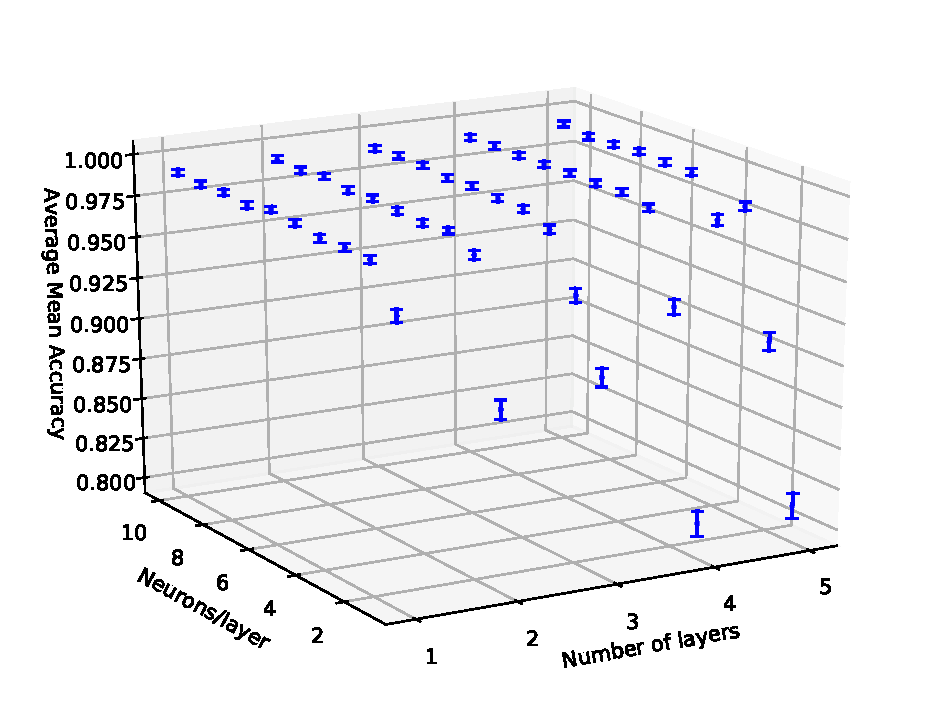
\includegraphics[width=0.9\linewidth]{../output/neural_network/figures/nn_architecture_global_standard_941_486}
		\caption{Correlation threshold: 1.0 (486 features)}
	\end{subfigure}
	\begin{subfigure}{0.5\linewidth}
		\centering
		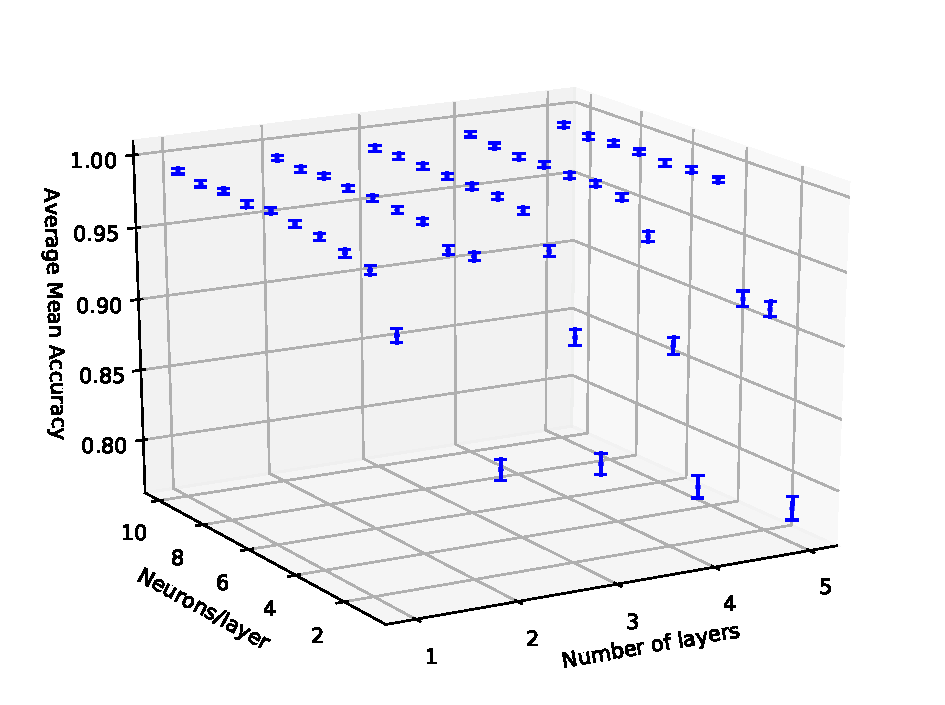
\includegraphics[width=0.9\linewidth]{../output/neural_network/figures/nn_architecture_global_standard_941_486_feature_pearson_99}
		\caption{Correlation threshold: 0.99 (195 features)}
	\end{subfigure}
	\begin{subfigure}{0.5\linewidth}
		\centering
		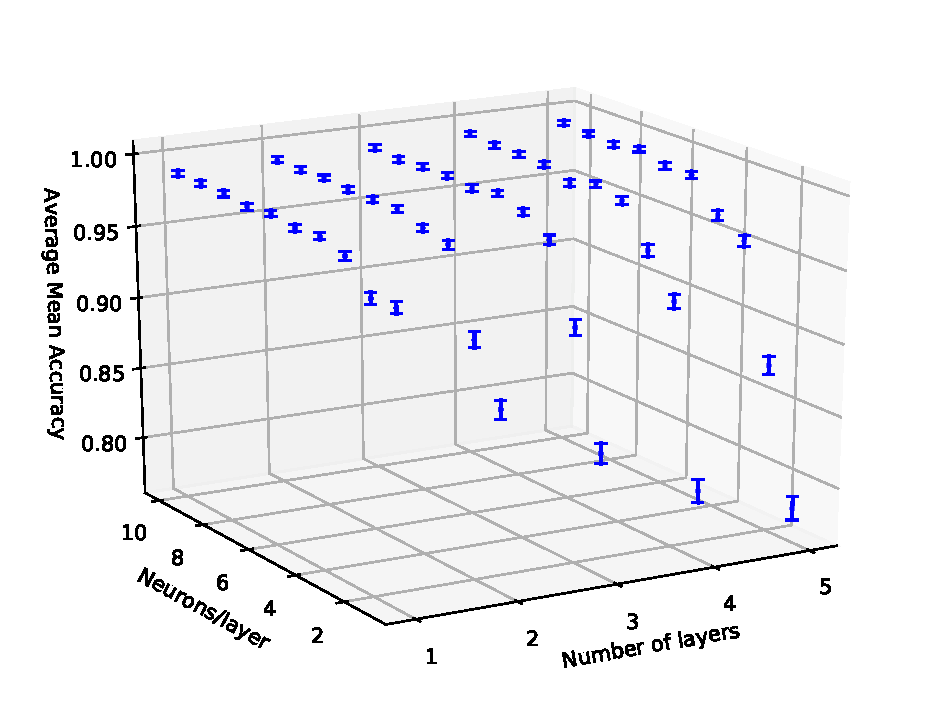
\includegraphics[width=0.9\linewidth]{../output/neural_network/figures/nn_architecture_global_standard_941_486_feature_pearson_90}
		\caption{Correlation threshold: 0.9 (101 features)}
	\end{subfigure}
	\begin{subfigure}{0.5\linewidth}
		\centering
		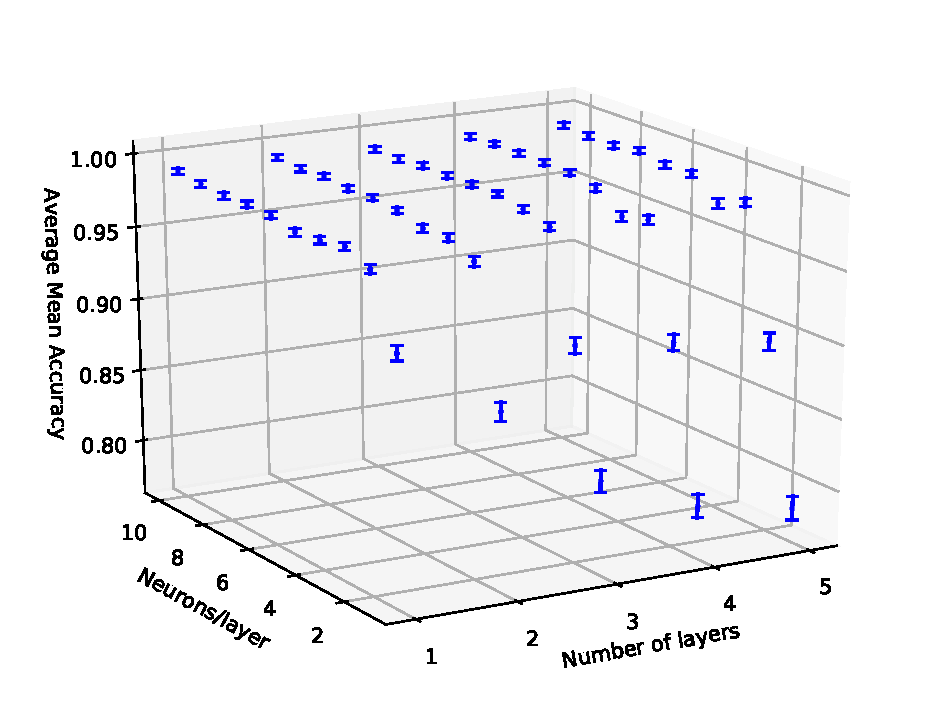
\includegraphics[width=0.9\linewidth]{../output/neural_network/figures/nn_architecture_global_standard_941_486_feature_pearson_80}
		\caption{Correlation threshold: 0.8 (70 features)}
	\end{subfigure}
	\caption{The average mean accuracy as function of the number of layers used, the number of neurons per layer and the correlation threshold.}
	\label{fig:nn_architecture_global_gauss}
\end{figure} 

All combinations showed similar behavior, thus for brevity, only the results in Figure \ref{fig:nn_architecture_global_gauss} are presented explicitly.
\\
\\
Next, the differences between stochastic, mini-bach, and batch learning algorithms are analyzed.
Here, the objective is to characterize the training performance in terms of epochs and time required for convergence. 
For this study, the architecture of the neural net is fixed to have 4 layers with 7 neurons per layer, since this is already in the domain where the differences between models are statistically insignificant.
Thus, for this study only the activation functions, input normalizations, batch sizes and correlation thresholds are changed.
The results for the global standard normalization are presented in Figure \ref{fig:nn_convergence_global_gauss}.
For all of the experiments the batch size goes from 1 to 621.
The reason behind this is that we use a single fold cross-validation to evaluate the model which is trained on $66\%$ of the data corresponding to 621 samples.
A batch size of 1 corresponds to a purely stochastic Adam gradient descend, while a batch size between 2 and 620 denotes mini-batch learning and 621 the regular batch learning, respectively.
Also, the results presented are average values obtained using 10 different random number seeds to reduce the statistical fluctuation.

\begin{figure}[H]
	\begin{subfigure}{0.5\linewidth}
		\centering
		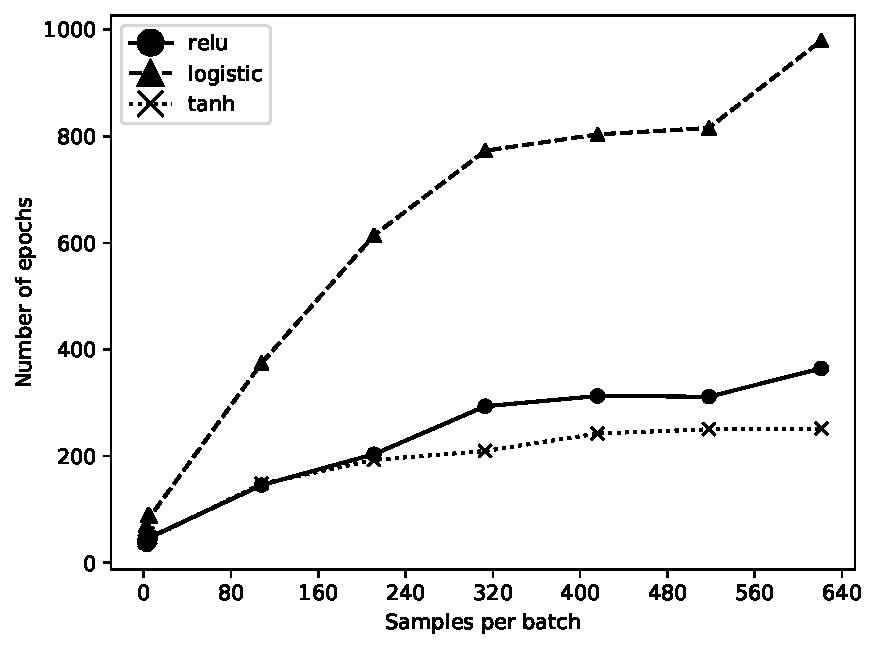
\includegraphics[width=0.8\linewidth]{../output/neural_network/figures/nn_convergence_global_standard_941_486}
		\caption{Correlation threshold: 1.0 (486 features)}
	\end{subfigure}
	\begin{subfigure}{0.5\linewidth}
		\centering
		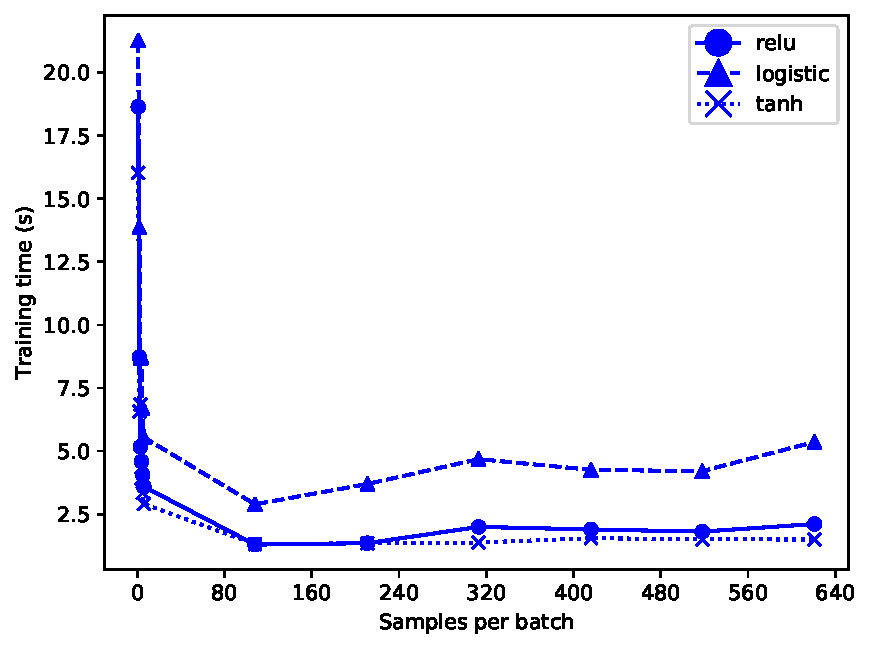
\includegraphics[width=0.8\linewidth]{../output/neural_network/figures/nn_convergence_global_standard_941_486_time}
		\caption{Correlation threshold: 1.0 (486 features)}
	\end{subfigure}
	\begin{subfigure}{0.5\linewidth}
		\centering
		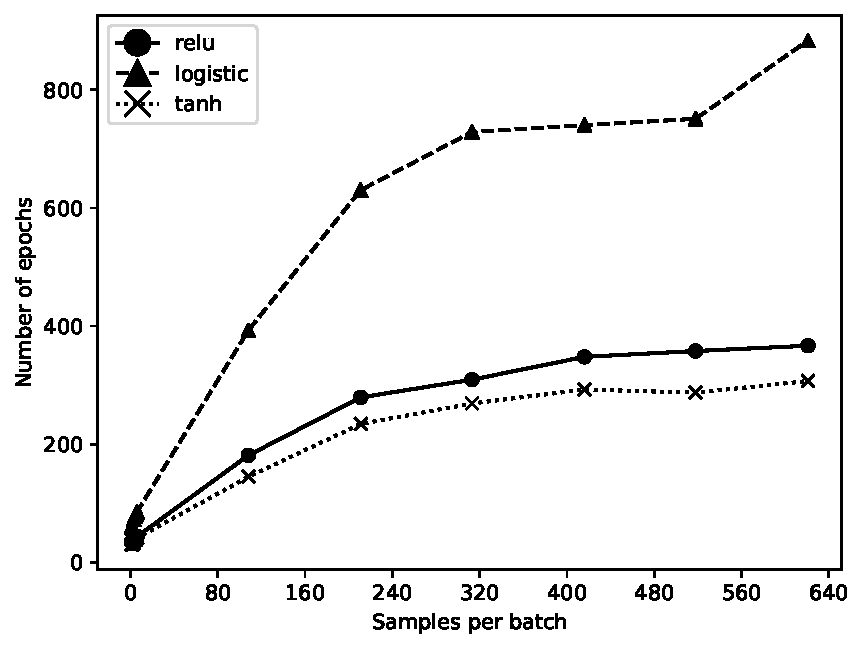
\includegraphics[width=0.8\linewidth]{../output/neural_network/figures/nn_convergence_global_standard_941_486_feature_pearson_90}
		\caption{Correlation threshold: 0.9 (101 features)}
	\end{subfigure}
	\begin{subfigure}{0.5\linewidth}
		\centering
		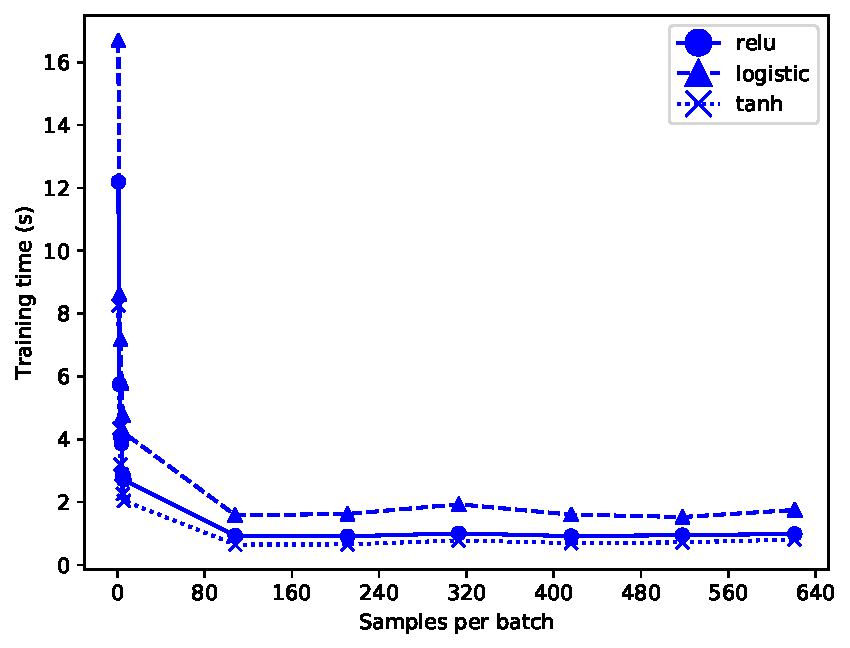
\includegraphics[width=0.8\linewidth]{../output/neural_network/figures/nn_convergence_global_standard_941_486_feature_pearson_90_time}
		\caption{Correlation threshold: 0.9 (101 features)}
	\end{subfigure}
	\caption{The number of epochs and training time until convergence as function of the batch size used for the training in case of global standardization.}
	\label{fig:nn_convergence_global_gauss}
\end{figure}  

It is clear that the stochastic gradient descent needs the fewest epochs for convergence. 
This result is consistent with what has been shown in the literature.
It is worth noting that while in terms of epochs the convergence rate is fastest, in computational cost, it is most expensive.
The reason behind this is that each epoch contain 621 weight updates. 
Due to the fact that the number of model parameters in this network is extensive (4408), updating them after every sample results in an unreasonable computational burden.
As the batch size increases, the number of iterations needed for convergence increases, however, the training time decreases.
For instance, using a batch size of two, half of the weight updates are required for a given epoch.
For a large network architecture, these savings can be tremendous.
From these results, it is clear that either the $tanh(x)$ or $ReLU(x)$ activation functions are the optimal choices.
While, the difference between $tanh(x)$ and $ReLU(x)$ is marginal, the logistic activation function clearly yields the slowest converging models.
Additionally, the reduction of train time due to the reduction in the input features is also seen.
In the case of purely stochastic learning, this reduction can be up to 20\%. 
The number of epochs needed for convergence decreases by 10-20\% as well.
Though this is an improvement, the reduction in the input parameters influences the number of parameters in the first hidden layer alone.
This means that when multiple hidden layers are present in the neural network, the gain becomes less and less.

For comparison, the results with time-step based input normalization are presented as well.
Figure \ref{fig:nn_convergence_time_gauss} shows the number of epochs and training time to convergence.

\begin{figure}[H]
	\begin{subfigure}{0.5\linewidth}
		\centering
		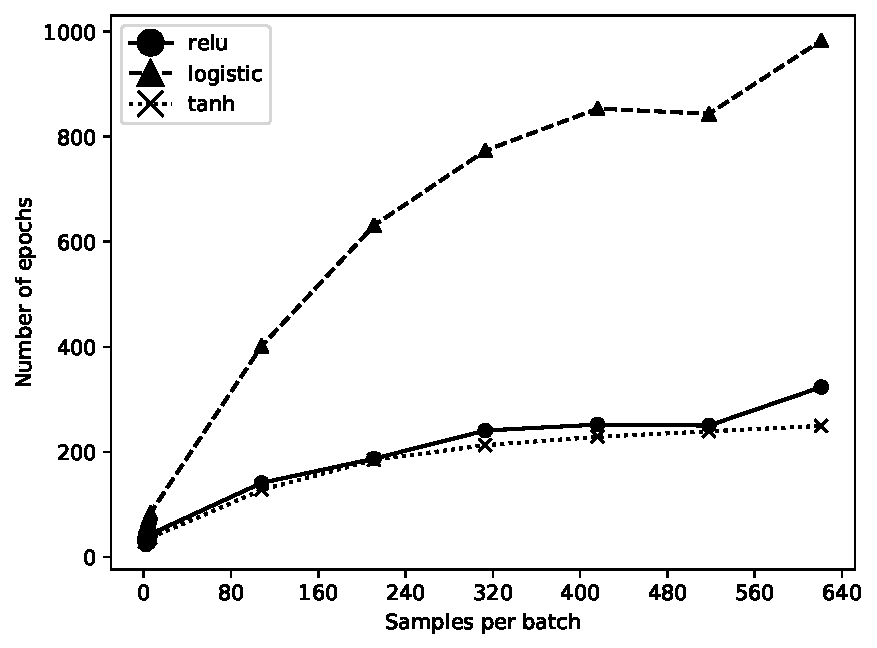
\includegraphics[width=0.8\linewidth]{../output/neural_network/figures/nn_convergence_time_standard_941_486}
		\caption{Correlation threshold: 1.0 (486 features)}
	\end{subfigure}
	\begin{subfigure}{0.5\linewidth}
		\centering
		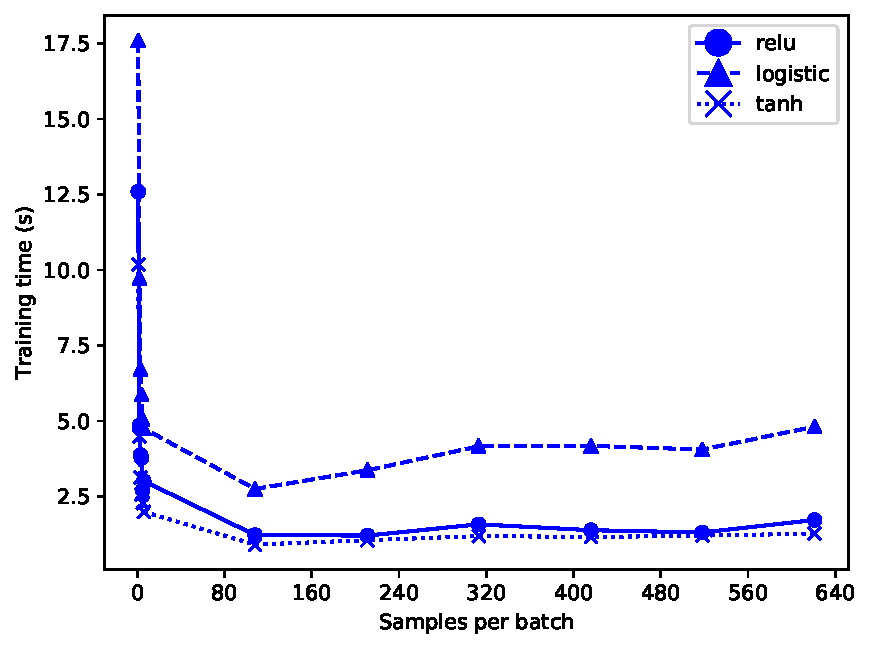
\includegraphics[width=0.8\linewidth]{../output/neural_network/figures/nn_convergence_time_standard_941_486_time}
		\caption{Correlation threshold: 1.0 (486 features)}
	\end{subfigure}
	\begin{subfigure}{0.5\linewidth}
		\centering
		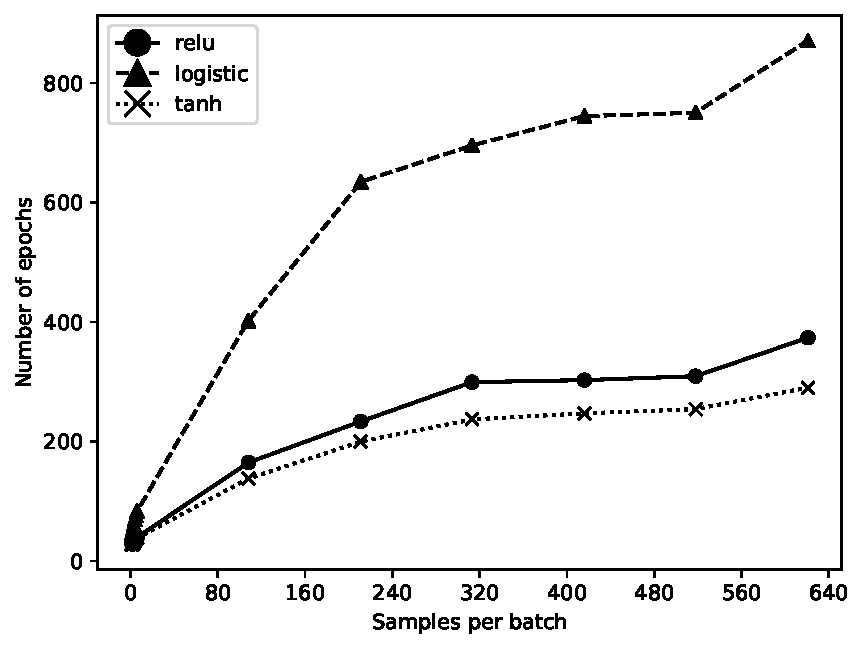
\includegraphics[width=0.8\linewidth]{../output/neural_network/figures/nn_convergence_time_standard_941_486_feature_pearson_90}
		\caption{Correlation threshold: 0.9 (101 features)}
	\end{subfigure}
	\begin{subfigure}{0.5\linewidth}
		\centering
		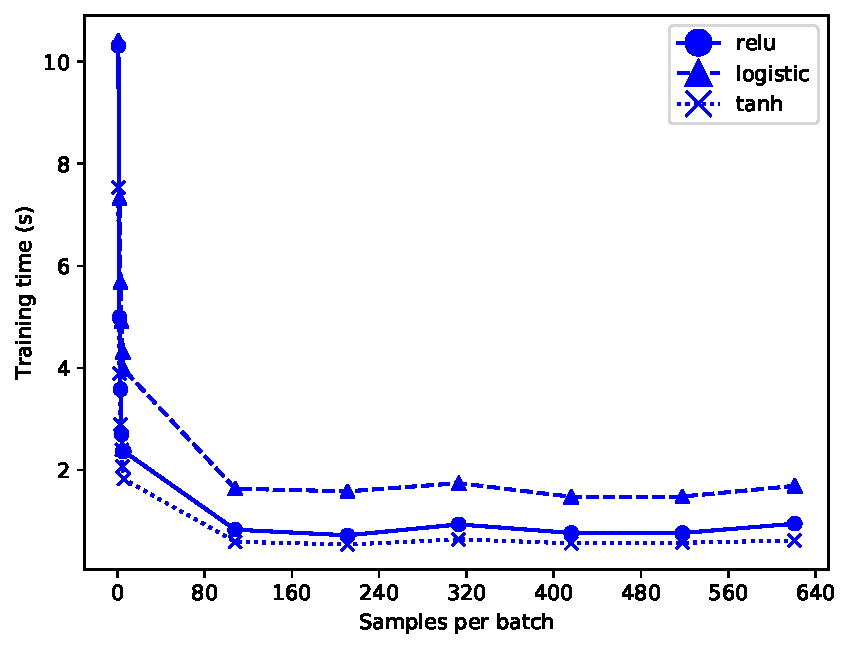
\includegraphics[width=0.8\linewidth]{../output/neural_network/figures/nn_convergence_time_standard_941_486_feature_pearson_90_time}
		\caption{Correlation threshold: 0.9 (101 features)}
	\end{subfigure}
	\caption{The number of epochs and training time until convergence as function of the batch size used for the training in case of time-step based standardization.}
	\label{fig:nn_convergence_time_gauss}
\end{figure} 

Overall, the results look similar to those with the global standard normalization with one important difference.
Namely, the training time for stochastic learning is 15-20\% less than in the previous result. 
As the batch size grows, the results with time-step normalization converge to the previous results.

\subsection*{Best Model Results}

From the aforementioned optimizations, the best models are selected and analyzed using three-fold cross-validation.
The metric for these comparisons is the mean average accuracy.
A ReLU activation function and a mini-batch learning with 200 samples is considered for all cases.
Table \ref{tab:best_nn_models_unfiltered} shows the results from the best models with different normalizations of the data-set without filtering the features based on the correlations.
By analyzing the mean values and the corresponding confidence intervals, it is apparent that the accuracies are statistically the same for all four normalizations.
\begin{table}[H]
	\small
	\centering
	\caption{Important statistics of the best neural network models with different data-set normalizations and without correlation filtering.}
	\label{tab:best_nn_models_unfiltered}
	\begin{tabular}{|c|c|c|c|c|}
		\hline
		\textbf{Normalization}         & \textbf{Global Stand.}        & \textbf{Global Max.}            & \textbf{Time Stand.}            & \textbf{Time Max.} \\ \hline \hline
		Number of layers     & 2                    & 3                      & 4                     & 1 \\ \hline
		Neurons per layer    & 9                    & 6                      & 8                     & 6 \\ \hline
		Mean Accuracy        & 0.9936               & 0.9926                 & 0.9915                & 0.9915 \\ \hline
		Standard Deviation   & 0.0026               & 0.0028                 & 0.0030                & 0.0030 \\ \hline
		95.00\% Confidence   & 0.9936 $\pm$ 0.0051  & 0.9926 $\pm$ 0.0055    & 0.9915 $\pm$ 0.0059   & 0.9915 $\pm$ 0.0059 \\ \hline
		Accuracy Range       & (0.9885, 0.9987)     & (0.9871, 0.9981)       & (0.9856, 0.9974)      & (0.9856, 0.9974) \\ \hline
		Best Accuracy        & 0.9968               & 0.9936                 & 0.9936                & 0.9936 \\ \hline
		Training Time        & 7.5350 s             & 13.4279 s              & 5.2132 s              & 8.6126 s \\ \hline
		Classification Time  & 0.0039 s             & 0.0078 s               & 0.0035 s              & 0.0025 s  \\ \hline
	\end{tabular}
\end{table}

It is also visible that subtracting the mean and normalizing with the variance (standardization) yields shorter training periods compared to models using the data-set normalized by the maximums.
A possible explanation for this can be that the algorithm manages to converge faster due to the less skewed loss function surface in the parameter space.
Following this, Table \ref{tab:best_nn_models_filtered} presents the important statistics for the best models that were obtained using filtering the correlated features. 
In this case a threshold of 0.9 is set for the Pearson correlation filter.
The results indicate that the accuracy slightly decreases when the correlation filter is applied. 
This change, however is statistically insignificant due to the overlapping confidence intervals.
For this reason, the utilization of the correlation filter can be a good approach to accelerate the training without a statistically significant loss in accuracy.

Since the accuracies are statistically the same for every case, the best model is selected to be the fastest to train.
The ones built using a snapshot-based standardization on the data-set perform the best in this sense.
The true and false positive/negative counts for this model across the 3 folds in the cross-validation are summarized in Table \ref{tab: cv_best_nn} for the non-filtered data-set and in Table \ref{tab: cv_best_nn_filtered} for the case with the correlation threshold set to 0.9.

\begin{table}[H]
	\small
	\centering
\caption{Important statistics of the best neural network models with different data-set normalizations and with the correlation filter set to 0.9.}
	\label{tab:best_nn_models_filtered}
	\begin{tabular}{|c|c|c|c|c|}
		\hline
		\textbf{Normalization }        & \textbf{Global Stand.}        & \textbf{Global Max.}            & \textbf{Time Stand.}            & \textbf{Time Max.} \\ \hline \hline
		Number of layers     & 4                    & 5                      & 2                     & 1 \\ \hline
		Neurons per layer    & 10                   & 7                      & 8                     & 7 \\ \hline
		Mean Accuracy        & 0.9894               & 0.9904                 & 0.9851                & 0.9830 \\ \hline
		Standard Deviation   & 0.0033               & 0.0032                 & 0.0039                & 0.0042 \\ \hline
		95.00\% Confidence   & 0.9894 $\pm$ 0.0066  & 0.9904 $\pm$ 0.0062    & 0.9851 $\pm$ 0.0077   & 0.9830 $\pm$ 0.0083 \\ \hline
		Accuracy Range       & (0.9828, 0.9959)     & (0.9842, 0.9967)       & (0.9774, 0.9929)      & (0.9747, 0.9913) \\ \hline
		Best Accuracy        & 0.9904               & 0.9936                 & 0.9904                & 0.9872 \\ \hline
		Training Time        & 4.8473 s             & 4.6460 s               & 4.0463 s              & 4.2933 s \\ \hline
		Classification Time  & 0.0025 s             & 0.0024 s               & 0.0021 s              & 0.0015 s  \\ \hline
	\end{tabular}
\end{table}

\begin{table}[H]
	\centering
	\caption{Cross-validation results for the tuned neural network using the unfiltered data-set and time-based standardization.}
	\begin{tabular}{|c|c|c|c|c|c|}
		\hline
		\textbf{Fold} & \textbf{TP} & \textbf{TN} & \textbf{FP} & \textbf{FN} & \textbf{Accuracy} \\ \hline \hline
		1 & 70 & 240 & 1 & 3 & 0.9873  \\ \hline
		2 & 70 & 242 & 0 & 2 & 0.9936  \\ \hline
		3 & 70 & 241 & 0 & 2 & 0.9936  \\ \hline
	\end{tabular}
	\label{tab: cv_best_nn}
\end{table}

\begin{table}[H]
	\centering
	\caption{Cross-validation results for the tuned neural network using a data-set  with correlation filtering and time-based standardization.}
	\begin{tabular}{|c|c|c|c|c|c|}
		\hline
		\textbf{Fold} & \textbf{TP} & \textbf{TN} & \textbf{FP} & \textbf{FN} & \textbf{Accuracy} \\ \hline \hline
		1 & 71 & 240 & 1 & 2 & 0.9904  \\ \hline
		2 & 69 & 238 & 4 & 3 & 0.9777  \\ \hline
		3 & 70 & 239 & 2 & 2 & 0.9872  \\ \hline
	\end{tabular}
	\label{tab: cv_best_nn_filtered}
\end{table}

\section{Novel Learner} \label{sec: novel}

\subsection*{Literature Review} 

When an ensemble model is to be designed, previous works in the field of machine learning have shown that decision trees, perceptrons and neural networks are the most commonly used weak learners. 
The naive Bayes classifier is a simple, probabilistic classifier that can be trained to be very accurate on real-world data.
The authors of \cite{ensemble-lit1} compare three algorithms for automated morphological galaxy classification with a sample of 800 galaxies:
\begin{enumerate}
	\item A naive Bayes classifier, 
	\item A neural network trained with back-propagation, 
	\item A decision-tree induction algorithm with pruning. 
\end{enumerate} 
The ensembles of classifiers were trained using 25 bootstrap data-sets.
The individual classifiers and their ensembles were both tested using the same 10-fold cross-validation test sets.
Their results showed that:
\begin{enumerate}
	\item The neural network produced the lowest classification error, 
	\item The ensemble approach significantly reduced the classification error for the neural network and the decision-tree classifiers, but not for the naive Bayes classifier, 
	\item The ensemble approach was better for decision trees than for the neural network.
\end{enumerate} 
A classifier is unstable if perturbing (modifying) the training set by removing some training examples and repeating others changes the final classifier.
This, by definition, is what occurs with a bootstrap approach.
Neural networks and decision trees have been found to be unstable in this sense, unlike the naive Bayes classifier.
The authors point out that if different classifiers within an ensemble perform well individually and their predictions are not correlated, then the combined outputs of the ensemble often will be more accurate than any of the individual classifiers.
As a result of this property, the authors saw a reduction in error rate for both the neural network and the decision tree when using bagged ensembles.
\\

The authors of \cite{ensemble-lit2} evaluate bagging and boosting methods on 23 data-sets using both neural networks and decision trees.
Their results indicate that bagging is sometimes much less accurate than boosting, however, boosting can create ensembles that are less accurate.
Breiman (1996) \cite{ensemble-lit3}, Bauer \& Kohavi (1999) \cite{ensemble-lit4}, Opitz \& Maclin (1999) \cite{ensemble-lit5}, and Dietterich (2000) \cite{ensemble-lit6} studied bagging as a method to create ensembles of classifiers and have shown it to be effective in decreasing classification errors for unstable learning algorithms.
\\

The novel learner used in this work uses an ensemble of decision trees whose outputs serve as the inputs to a neural network. 
The hypothesis is that the neural network will outperform the previous novel learner, which used a perceptron in lieu of the neural network, by virtue of being able to learn how to best aggregate the outputs of the ensemble of decision trees in a nonlinear way.
Additionally, the authors believe that by using the decision tree as a filter, several advantages over using only a neural network are obtained, namely:
\begin{enumerate}
	\item The decision tree outputs map the neural network input to binary, making the neural network performance less sensitive to the input transformation applied.
	\item By using the decision tree ensemble, some of the underlying structures are encoded in the inputs to the neural network, thus simplifying the underlying target function. This would result in smaller required network size for comparable or better accuracy, and necessarily, a faster training time.
\end{enumerate}


\subsection*{Algorithm}

A depiction of the novel learner design is shown in Figure \ref{fig: novel}.

\begin{figure}[H]
	\begin{center}
		\makebox[\linewidth][c]{	
			\begin{tikzpicture}[scale=0.5]
			% get node at origin
			% variable definitions
			\def\s{5.}; % size of each DT input square
			\def\vertOffset{0.5*\s}; % distance to offset next box above previous
			\def\r{0.75*\s}; % perceptron radius
			\def\d{4*\s}; % distance between inputs and perceptron
			\def\picWidth{3.0};
			
			% draw perceptron
			\draw[fill=cyan] (\d, 0) circle (\r) node {Neural Network};
			
			% draw bias
			\def\i{2};

			% draw DTs
			\draw (0.5*\s, 0) circle (0.0) node {\vdots};
			\foreach \i / \ID / \j in {2/0/0 ,1/1/1, -1/2/N-1, -2/13/N}
			{
				% insert tree
				\node at (0.5*\s, {\i*(\s + \vertOffset)}) {\includegraphics[width=2.8cm]{../output/PF/PF_941_486/PF_DT\ID_best.gv.pdf}};
				\node[anchor=south] at (0.5*\s, {\i*(\s + \vertOffset) + 0.5*\s}) {$x_{\j}$};
				% put box around tree
				\draw (0, {\i*(\s + \vertOffset) - 0.5*\s}) rectangle (\s, {\i*(\s + \vertOffset) + 0.5*\s});
				% draw line from box to perceptron
				\draw (\s, {\i*(\s + \vertOffset)}) -- (\d-\r,0);
				% label line with weight
			}
			\end{tikzpicture}
	}
	\caption{Diagram of the novel ensemble network.}
	\label{fig: novel}
	\end{center}
\end{figure}

The learner is an ensemble model which uses a neural network to aggregate the votes of each of the weak learners.
As suggested by the literature, using unstable weak learners in an ensemble yields optimal accuracy.
For this reason, decision trees are used as the ensemble.
The algorithms utilized for each of these components are those from Scikit-Learn.
The neural network algorithm is discussed in Section \ref{sec: neural net} and the decision tree and ensemble algorithms in Zach and Patrick's homework two report.
\\

Three objects are used in the implementation of this algorithm
\begin{enumerate}
	\item \verb|DecisionTree|, an interface to Scikit-Learn's \verb|DecisionTreeClassifier| object,
	\item \verb|BaggingClassifier|, a Scikit-Learn object for ensembles of weak learners,
	\item \verb|NeuralNetwork|, an interface to Scikit-Learn's \verb|MLPClassifier| (Multi-Layer Percepton) object.
\end{enumerate}
The \verb|BaggingClassifier| contains the ensemble of \verb|DecisionTree| objects.
The hyper-parameters of the decision trees are specifically chosen to enable over-fitting using the subset of the data they are trained with.
The primary hyper-parameters governing the ensemble are the number of weak estimators, \verb|n_estimators|, and the fraction of data passed to each of them.
Additionally, options to train the ensemble with or without replacement are available.
\\

To train this model, the standard \verb|fit| method can be called.
This method takes in the training samples and corresponding labels.
Initially, the ensemble is fit using the \verb|fit| method of Scikit-Learn's \verb|BaggingClassifier| object.
This constructs \verb|n_estimators| \verb|DecisionTree| objects based upon the subsets of the data internally passed to them.
After this, the training data is passed through the ensemble model to form the input to the neural network.
This input is of dimension \verb|n_estimators| and is binary.
The neural network is then trained on this data in the same fashion as described in Section \ref{sec: neural net}.
To use the learner, the \verb|predict| method is can be called similarly to all other models.
The input samples are evaluated by each of the decision trees using \verb|BaggingClassifier|'s \verb|predict| method and the subsequent classification results are passed to the \verb|predict| method of the neural network.
\\

In general, this overall design aims to maintain or improve upon the accuracy of the neural network while reducing the overall training cost by using a decision tree ensemble as a filter to:
\begin{enumerate}
	\item Simplify the input to binary,
	\item Reduce the input dimensionality to the neural network,
	\item Simplify the target function the neural network must learn.
\end{enumerate}
To achieve this goal, it is clear that the savings in training the neural network with the ensemble filtered data must outweigh the cost of training the ensemble model.
This implies that an optimal model will use the smallest architecture and number of weak learners.
The savings from this learner are expected to be problem dependent.


\subsection*{Model Complexity}

Suppose $N$ is the number of samples, $n$ is the number of trees in the ensemble, $k$ is the number of samples passed to each tree, and $D$ is the number of features, $I$ is the number of epochs needed for convergence, $H$ is the number of neurons per hidden layer, and $L$ is the number of layers.
It is assumed that all layers of the neural network have an equivalent number of neurons and the stochastic gradient descent is used for training.
To determine the time complexity of training this algorithm, the complexity of each step is discussed:
\begin{itemize}
	\item[(1)] 
	Training samples are drawn with replacement into $n$ sub-sets of $k$ samples.
	Each subset is used to train a decision tree.
	The process of building one tree costs between $\mathcal{O}\left( D k \log k \right)$ and  $\mathcal{O} \left(D k^2 \log k \right)$. 
	Refer to decision tree sub-section of the complexity section of Zach, Patrick, Jiacong, and Hanzhou's homework three report to get the detailed discussion.
	Therefore, building $n$ trees costs between $\mathcal{O} \left( n D k \log k \right)$ and \\ $\mathcal{O} \left( n D k^2 \log k \right)$.
	
	\item[(2)] 
	$n$ trees built on subsets of the data-set are used to predict samples' labels to be input to the perceptron.
	This then costs the same as $n$ decision tree evaluations, bounded by $\mathcal{O} \left( \log k \right)$ and $\mathcal{O} \left( k \right)$.
	The cost of this for $N$ samples is then between $\mathcal{O} \left( N n \log k \right)$ and $\mathcal{O} \left( N n k \right)$.
	The cost up to now is then between $\mathcal{O} \left( n D k \log k + N n \log k \right)$ and \\ $\mathcal{O} \left( n D k^2 \log k + N n k \right)$.
	
	\item[(3)] 
	Because the decision tree classifications will not change after evaluated once, these can be stored.
	The cost of the neural network is the same cost as discussed in Section \ref{sec: neural net}, where the number of inputs is the number of trees, $n$. 
	The cost of training the neural network is then $\mathcal{O}\left(I  N \left[n  H + H^{L-1} + O H \right]\right)$.
	This gives a total training cost between \\ $\mathcal{O} \left( n D k \log k + N n \log k + I N \left[ n H + H^{L-1} + O H \right] \right)$ and \\ $\mathcal{O} \left( n D k^2 + N n k + I N \left[ n H + H^{L-1} + O H \right]\right)$
\end{itemize}

For predictions, the cost is simply the cost of evaluating $n$ decision trees and a forward pass of those results through the neural network.
This ranges between \\ $\mathcal{O} \left( n \log k + n H + H^{L-1} + O H \right)$ and $\mathcal{O} \left( n k + n H + H^{L-1} + O H \right)$.

\subsection*{Optimizations}

This section outlines the optimizations employed to find the best hyper-parameters for the novel ensemble network.
The primary hyper-parameters of interest are:
\begin{enumerate}
	\item The architecture of the neural network,
	\item The number of weak learners in the ensemble.
\end{enumerate}
With the goal of reducing the training time relative to the neural network, it is important to limit the network architecture size and number of weak learners in the ensemble.
For this reason the network size was held to a maximum of three layers with no more than eight neurons in each layer.
For simplicity, each layer contains the same number of neurons.
Grid searches were performed for each normalization method with no correlation and a correlation threshold of 0.9.
For brevity, and due to the similarity in all results, only results for global and time standardization are shown with and without filtering.
Each result was obtained using ten decision trees in the ensemble.
This is shown in Figure \ref{fig:en_architecture_global}.

\begin{figure}[H]
		\begin{subfigure}{0.5\linewidth}
			\centering
			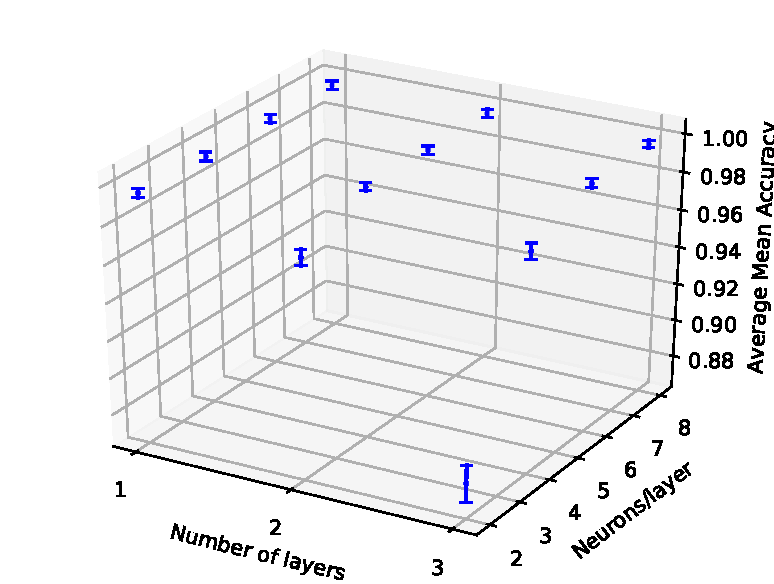
\includegraphics[width=\linewidth]{../output/EN/figures/en_architecture_global_standard_941_486_N10.pdf}
            \caption{Global standardization with no filtering.}
		\end{subfigure}
		\begin{subfigure}{0.5\linewidth}
			\centering
			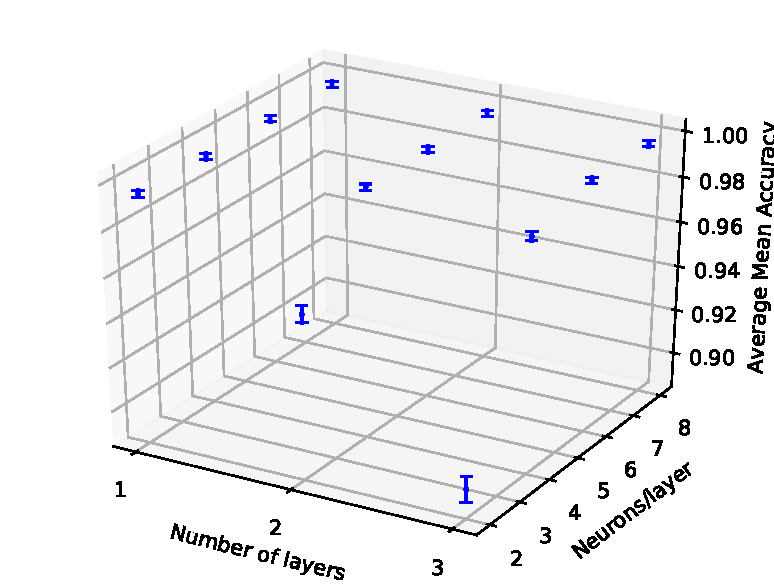
\includegraphics[width=\linewidth]{../output/EN/figures/en_architecture_global_standard_941_486_feature_pearson_90_N10.pdf}
			\caption{Global standardization with filtering.}
		\end{subfigure}
		\begin{subfigure}{0.5\linewidth}
			\centering
			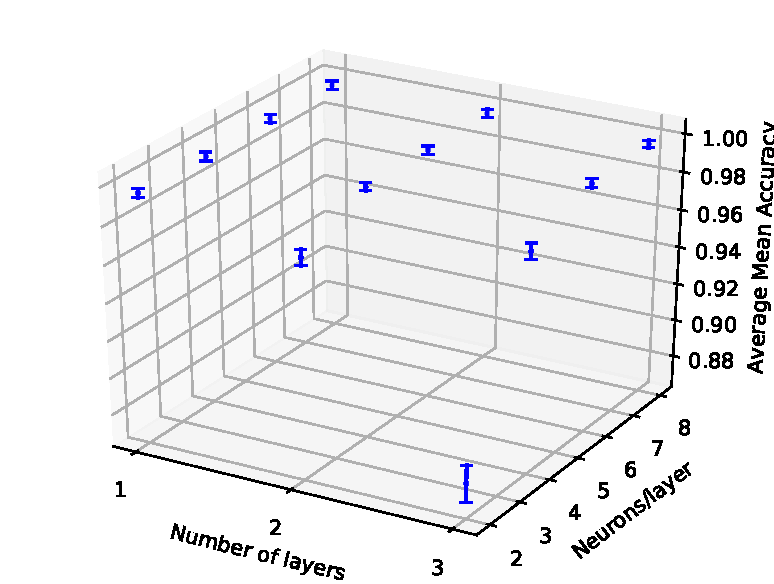
\includegraphics[width=\linewidth]{../output/EN/figures/en_architecture_time_standard_941_486_N10.pdf}
			\caption{Time standardization with no filtering.}
		\end{subfigure}
		\begin{subfigure}{0.5\linewidth}
			\centering
			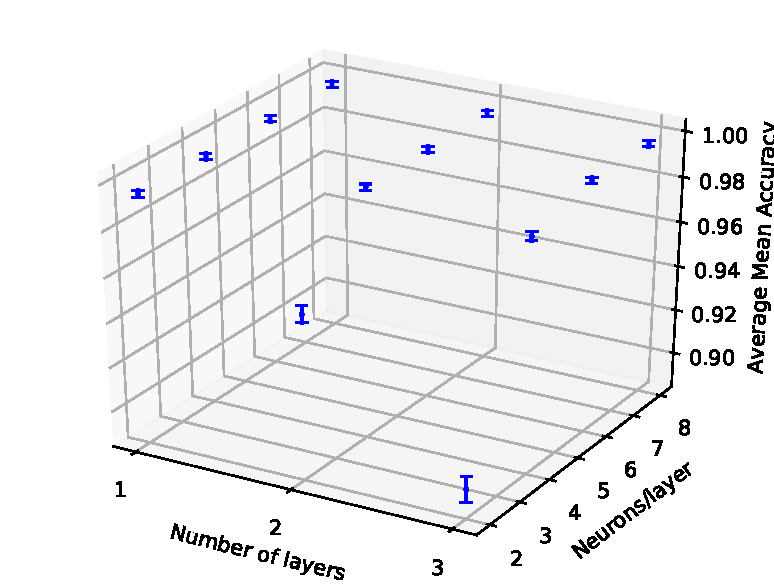
\includegraphics[width=\linewidth]{../output/EN/figures/en_architecture_time_standard_941_486_feature_pearson_90_N10.pdf}
			\caption{Time standardization with filtering.}
		\end{subfigure}
         \caption{Accuracy vs. architecture for a fixed ensemble size.}
         \label{fig:en_architecture_global}                     
\end{figure}

Results for the global and time-based maximum normalization methods were similar to this.
Additionally, the results for different numbers of estimators were more or less the same.
It is apparent that the results are not sensitive to the normalization used.
This is largely due the ensemble acting as a filter, mapping the input to binary values.
It is also apparent that light correlation filtering leads to comparable results.
Another interesting observation is that good performance is observed across all normalization types and filter values using only a single layer and that as in the plain neural network, a saturation is achieved once about four neurons per layer is reached.
Similar to the result in Section \ref{sec: neural net}, an accuracy plateau is observed once the number of neurons per layers grows larger than about four.
To err on the side of conservatism, the optimal model is chosen to be one near the middle of the plateau with the smallest input dimension (with filtering).
\\

\subsection*{Best Model Results}

In this section, several different results will be presented to highlight the performance of the novel learner, relative the the neural network.
First, the results from the best models for each normalization are presented.
Next, results from the same architecture as the optimal neural network found in Section \ref{sec: neural net} are presented for comparison.
Lastly, results for more compact ensemble networks are presented.
\\

Results for the best models with no filtering for each normalization are shown in Table~\ref{tab: novel best}.

\begin{table}[H]
	\centering\small
	\caption{Important statistics of the best novel ensemble networks with different data-set normalization techniques without correlation filtering.}
	\begin{tabular}{|c||c|c|c|c|}
		\hline
		\textbf{Normalization} & \textbf{Global Stand.} & \textbf{Global Max.} & \textbf{Time Stand.} & \textbf{Time Max.} \\ \hline \hline
		\# of layers & 3 & 3 & 3 & 3 \\ \hline
		Neurons per layer & 8 & 8 & 8 & 6 \\ \hline	
		\# of estimators & 10 & 10 & 10 & 10 \\ \hline
		Mean Accuracy & 0.9957 & 0.9968 & 0.9777 & 0.9841 \\ \hline
		Standard Deviation & 0.0021 & 0.0018 & 0.0048 & 0.0041 \\ \hline
		95.00\% Confidence & 0.9957 $\pm$ 0.0067 & 0.9968 $\pm$ 0.0036 & 0.9777 $\pm$ 0.0094 & 0.9841 $\pm$ 0.0080 \\ \hline
		Accuracy Range & (0.9890, 1.0000) & (0.9932, 1.0000) & (0.9683, 0.9871) & (0.9761, 0.9920) \\ \hline
		Best Accuracy & 1.0000 & 1.0000 & 0.9841 & 0.9936 \\ \hline
		Training Time & 1.9466 s & 1.8837 s & 4.0080 s & 3.0748 s \\ \hline
		Classification Time & 0.0087 s & 0.0083 s & 0.2234 s & 0.2210 s \\ \hline
	\end{tabular}
	\label{tab: novel best}
\end{table}

It is clear that the plateau described earlier slopes upwards based on these results, however, the accuracy is close enough to unity that there is no statistical difference between many of the models in this range.
This will be shown later in the section when discussing results from more compact models.
From these results, it is clear that global normalization is optimal in terms of classification accuracy and training and test times.
The discrepancy in training and classification time is largely due to the complexity in the transformations that must be applied to the incoming data for time-based normalization.
\\

To compare performance on comparable network architectures, the novel ensemble network is run with the optimal architecture found in Section \ref{sec: neural net}.
This is shown in Table \ref{tab: novel compare}.

\begin{table}[H]
	\centering
	\caption{Comparison of ensemble network performance on optimal architecture for the neural network. The architecture is fixed to two layers with nine neurons and the ensemble network uses eight decision trees.}
	\begin{tabular}{|c||c|c|}
		\hline
		\textbf{Model} & \textbf{Neural Network} & \textbf{Ensemble Network} \\ \hline \hline
		Mean Accuracy & 0.9936 & 0.9979 \\ \hline
		Standard Deviation & 0.0026 & 0.0015 \\ \hline
		95.00\% Confidence & 0.9936 $\pm$ 0.0051 & 0.9979 $\pm$ 0.0048   \\ \hline
		Accuracy Range & (0.9885, 0.9987) & (0.9931, 1.0000) \\ \hline
		Best Accuracy  & 0.9968 & 1.0000 \\ \hline
		Training Time & 7.5350 s & 1.3033 s \\ \hline
		Classification Time & 0.0039 s &  0.0092 s \\ \hline
	\end{tabular}
	\label{tab: novel compare}
\end{table}

The performance of the model over the cross-validation suite is shown in Table \ref{tab: cv novel compare}.

\begin{table}[H]
	\centering
	\caption{Cross-validation results for the novel ensemble network on the data-set with correlation filtering and global standardization.}
	\begin{tabular}{|c|c|c|c|c|c|}
		\hline
		\textbf{Fold} & \textbf{TP} & \textbf{TN} & \textbf{FP} & \textbf{FN} & \textbf{Accuracy} \\ \hline \hline
		1 & 72 & 241 & 0 & 1 & 0.9968  \\ \hline
		2 & 72 & 241 & 1 & 0 & 0.9968  \\ \hline
		3 & 72 & 239 & 2 & 0 & 0.9936  \\ \hline
	\end{tabular}
	\label{tab: cv novel compare}
\end{table}

From this and the previous result, there is strong evidence to support that the ensemble network accomplishes its goal of improving upon the training time of the neural network with statistically comparable to better accuracy.
This result is most likely attributed to the ensemble filtering the input to significantly smaller dimension and simplifying the target function the network has to learn.
The clear pitfall of the ensemble network is its increased classification time as a result of needing to evaluate inputs on the ensemble of decision trees before a forward pass through the network.
Potential savings could be achieved if run in parallel.
\\

To demonstrate the insensitivity to architecture, several model evaluations are performed with smaller architectures.
As seen in Figure \ref{fig:en_architecture_global}, a single layer can yield good results even with a small number of neurons.
Results for a single layer with eight neurons and four decision trees is shown in Table \ref{tab: novel compact}.

\begin{table}[H]
	\centering
	\caption{Results for a compact novel ensemble network.}
	\begin{tabular}{|c||c|}
		\hline
		\textbf{Quantity} & \textbf{Value} \\ \hline \hline
		Mean Accuracy        & 0.9947 \\ \hline
		Standard Deviation   & 0.0024 \\ \hline
		95.00\% Confidence   & 0.9947 $\pm$ 0.0046 \\ \hline
		Accuracy Range       & (0.9900, 0.9993) \\ \hline
		Best Accuracy        & 0.9968 \\ \hline
		Training Time        & 1.2498 s\\ \hline
		Classification Time  & 0.0054 s \\ \hline
	\end{tabular}
	\label{tab: novel compact}
\end{table}

These architectures are obviously problem dependent, however, this result shows that with a single layer and very few estimators, the neural network can be considerably outperformed in terms of training time without degrading accuracy.
Further, with smaller architectures, the gap in classification time previously observed diminishes.
A breakdown of the model per cross-validation fold is shown in Table \ref{tab: cv compact novel}.
\begin{table}[H]
	\centering
	\caption{Cross-validation results for the compact novel ensemble network on the data-set with correlation filtering and global standardization.}
	\begin{tabular}{|c|c|c|c|c|c|}
		\hline
		\textbf{Fold} & \textbf{TP} & \textbf{TN} & \textbf{FP} & \textbf{FN} & \textbf{Accuracy} \\ \hline \hline
		1 & 73 & 239 & 2 & 0 & 0.9936  \\ \hline
		2 & 72 & 241 & 1 & 0 & 0.9968  \\ \hline
		3 & 72 & 239 & 2 & 0 & 0.9936  \\ \hline
	\end{tabular}
	\label{tab: cv compact novel}
\end{table}


\section{Old Model Comparison} \label{sec: compare}

Scikit-Learn's \verb|GridSearchCV| class was used to choose the optimal values for hyper-parameters given the model.
The Scikit-Learn interfaces are constructed in such a way that the \verb|GridSearchCV| class is compatible for models that combine several different learners. 
This method returns the combination of hyper-parameter values which produces the least error (or loss) on the test data. 
The best combination of values is then used to train the specific models.
\\


The old models from previous assignments are now optimized. The global standard normalization was used for all results as it produces the highest accuracy. Additionally, no correlation filtering was utilized.


\subsection*{Decision Tree}
Three decision tree hyper-parameters were varied to discover the perturbation yielding the highest mean cross-validation accuracy.
These parameters were the splitting criterion (\verb|entropy| or \verb|gini|), the maximum allowable depth of the tree (\verb|max_depth|, a crude form of pruning), and the cost complexity pruning parameter (\verb|ccp_alpha|).
Figure \ref{fig: tree grid} shows the resulting accuracy for the grid of hyper-parameters.
The highest accuracy results when the depth of the tree is not restricted and no cost complexity pruning is performed, indicating that over-fitting is not an issue with this data-set.
Thus, the optimal hyper-parameters are \verb|max_depth| = None and \verb|ccp_alpha| = 0.0.
Since both the entropy and gini criteria gave the same best accuracy, the value of this hyper-parameter did not matter and entropy was chosen.
The performance of the decision tree using these hyper-parameters is summarized in Table \ref{tab: cv best tree} and \ref{tab: best tree}.

\begin{figure}[H]
	\centering
	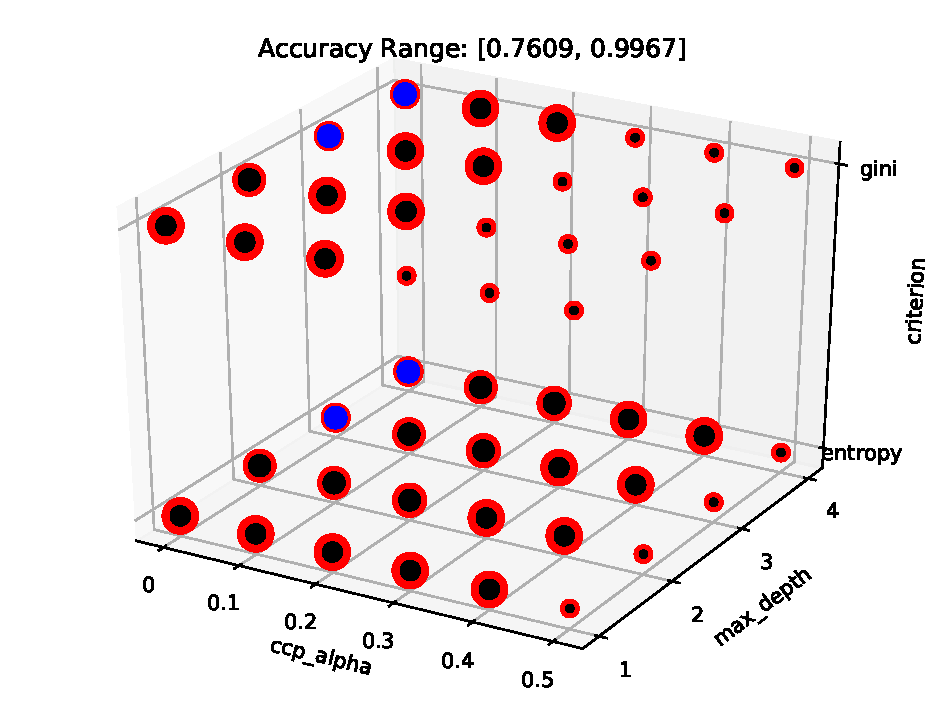
\includegraphics[scale=0.6]{../output/DT/DT_941_486/DT_gridsearch_941_486_global_standard.pdf}
	\caption{Hyper-parameter grid search for decision tree parameter tuning.
		The size of a point is proportional to it's accuracy, with the accuracy range of points given at the top of the plot.
		The points with the highest (statistically equivalent) accuracies are plotted in blue with all others plotted in black.
		The red outline around each point indicates the magnitude of the confidence interval relative to the point's accuracy.
		An outline twice the size of the point indicates a confidence interval of 0.2\%, one of three times the size of the point, a confidence interval of 0.4\%, etc..
		The grid search was performed using ten times repeated stratified ten-fold cross-validation.}
	\label{fig: tree grid}
\end{figure}

\begin{table}[H]
	\centering
	\caption{Three-fold cross-validation results for tuned decision tree.}
	\begin{tabular}{|c|c|c|c|c|c|}
		\hline
		\textbf{Fold} & \textbf{TP} & \textbf{TN} & \textbf{FP} & \textbf{FN} & \textbf{Accuracy} \\ \hline \hline
		1 & 72 & 240 & 1 & 1 & 0.9936  \\ \hline
		2 & 72 & 240 & 2 & 0 & 0.9936  \\ \hline
		3 & 71 & 241 & 0 & 1 & 0.9968  \\ \hline
	\end{tabular}
	\label{tab: cv best tree}
\end{table}

\begin{table}[H]
	\centering
	\caption{Performance results for tuned decision tree.}
	\begin{tabular}{|c|c|}
		\hline
		\textbf{Quantity}    & \textbf{Value}       \\ \hline \hline
		Mean Accuracy        & 0.9947 \\ \hline
		Standard Deviation   & 0.0024 \\ \hline
		95.00\% Confidence   & 0.9947 $\pm$ 0.0075 \\ \hline
		Accuracy Range       & (0.9871, 1.0000) \\ \hline
		Best Accuracy        & 0.9968 \\ \hline
		Training Time        & 0.2110 s\\ \hline
		Classification Time  & 0.0043 s \\ \hline
	\end{tabular}
	\label{tab: best tree}
\end{table}

\subsection*{Perceptron}
Two hyper-parameters were explored for the perceptron model: the type of regularization, or \verb|penalty|, and the corresponding regularization coefficient \verb|alpha|.
The resulting grid search is shown in Figure \ref{fig: perceptron grid}.
No regularization is chosen as the best option, again indicating that this model does not over-fit the data.
The performance of the perceptron using these hyper-parameters is summarized in Table \ref{tab: cv best perceptron} and \ref{tab: best perceptron}.

\begin{figure}[H]
	\centering
	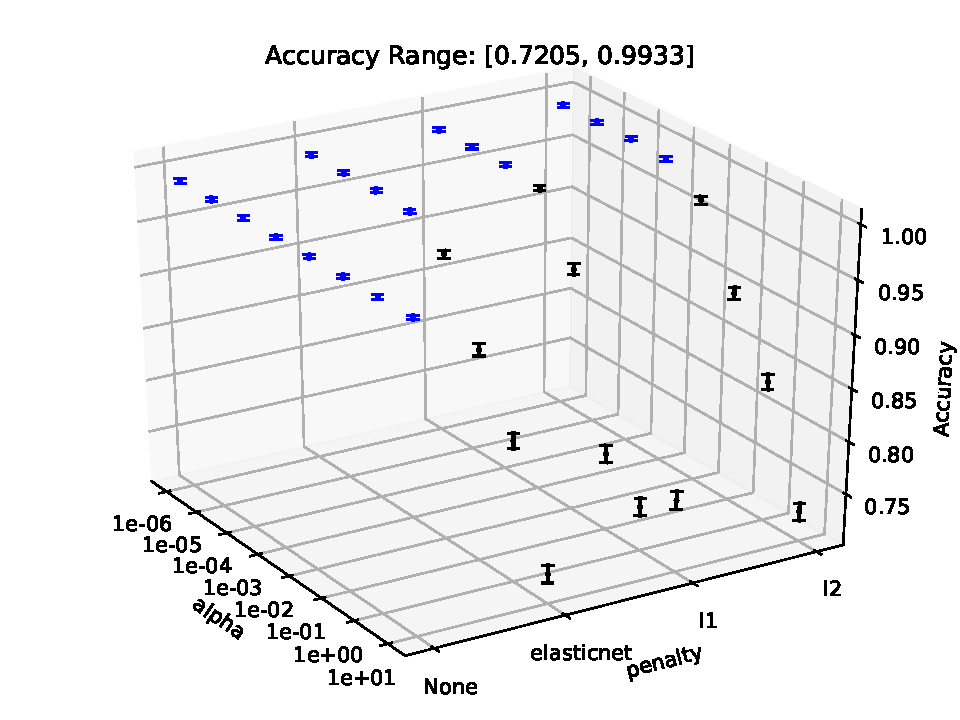
\includegraphics[scale=0.6]{../output/Perceptron/P_941_486/P_gridsearch_941_486_global_standard.pdf}
	\caption{Hyper-parameter grid search for perceptron parameter tuning.
		The points with the highest (statistically equivalent) accuracies are plotted in blue with all others plotted in black.
		The grid search was performed using ten times repeated stratified ten-fold cross-validation.}
	\label{fig: perceptron grid}
\end{figure}

\begin{table}[H]
	\centering
	\caption{Three-fold cross-validation results for tuned perceptron.}
	\begin{tabular}{|c|c|c|c|c|c|}
		\hline
		\textbf{Fold} & \textbf{TP} & \textbf{TN} & \textbf{FP} & \textbf{FN} & \textbf{Accuracy} \\ \hline \hline
		1 & 71 & 241 & 0 & 2 & 0.9936  \\ \hline
		2 & 72 & 240 & 2 & 0 & 0.9936  \\ \hline
		3 & 71 & 239 & 2 & 1 & 0.9904  \\ \hline
	\end{tabular}
	\label{tab: cv best perceptron}
\end{table}

\begin{table}[H]
	\centering
	\caption{Performance results for tuned perceptron.}
	\begin{tabular}{|c|c|}
		\hline
		\textbf{Quantity}    & \textbf{Value}       \\ \hline \hline
		Mean Accuracy        & 0.9926 \\ \hline
		Standard Deviation   & 0.0028 \\ \hline
		95.00\% Confidence   & 0.9926 $\pm$ 0.0055 \\ \hline
		Accuracy Range       & (0.9871, 0.9981) \\ \hline
		Best Accuracy        & 0.9936 \\ \hline
		Training Time        & 0.0450 s\\ \hline
		Classification Time  & 0.0033 s \\ \hline
	\end{tabular}
	\label{tab: best perceptron}
\end{table}

\subsection*{Perceptron Forest}
Both the number of trees \verb|n_estimators| feeding the perceptron and the fraction \verb|max_samples| of total training data presented to each tree was varied to find the best hyper-parameters.
Figure \ref{fig: perc forest grid} shows the corresponding grid search.
The parameters chosen result in two decision trees each trained on 20\% of the training data.
This is the best hyper-parameter combination that minimizes the amount of data required to train the trees, resulting in higher efficiency over other combinations.
The performance of the perceptron forest using these hyper-parameters is summarized in Table \ref{tab: cv best perceptron forest} and \ref{tab: best perceptron forest}.

\begin{figure}[H]
	\centering
	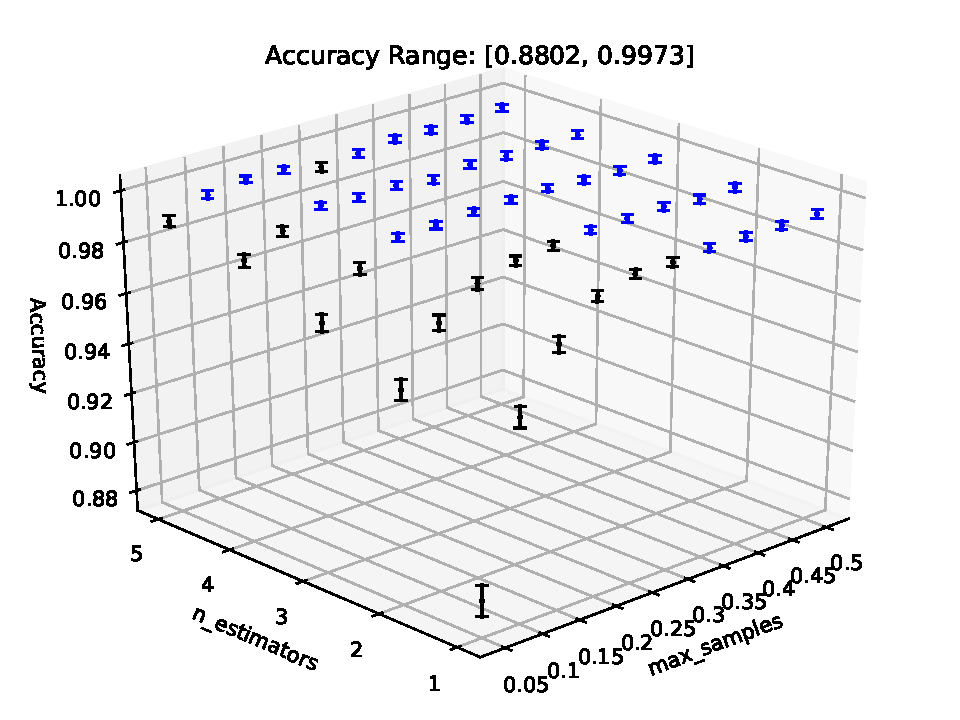
\includegraphics[scale=0.6]{../output/PF/PF_941_486/PF_gridsearch_941_486_global_standard.pdf}
	\caption{Hyper-parameter grid search for perceptron forest parameter tuning.
		The points with the highest (statistically equivalent) accuracies are plotted in blue with all others plotted in black.
		The grid search was performed using ten times repeated stratified ten-fold cross-validation.}
	\label{fig: perc forest grid}
\end{figure}

\begin{table}[H]
	\centering
	\caption{Three-fold cross-validation results for tuned perceptron forest.}
	\begin{tabular}{|c|c|c|c|c|c|}
		\hline
		\textbf{Fold} & \textbf{TP} & \textbf{TN} & \textbf{FP} & \textbf{FN} & \textbf{Accuracy} \\ \hline \hline
		1 & 72 & 241 & 0 & 1 & 0.9968  \\ \hline
		2 & 72 & 242 & 0 & 0 & 1.0000  \\ \hline
		3 & 72 & 241 & 0 & 0 & 1.0000  \\ \hline
	\end{tabular}
	\label{tab: cv best perceptron forest}
\end{table}

\begin{table}[H]
	\centering
	\caption{Performance results for tuned perceptron forest.}
	\begin{tabular}{|c|c|}
		\hline
		\textbf{Quantity}    & \textbf{Value}       \\ \hline \hline
		Mean Accuracy        & 0.9989 \\ \hline
		Standard Deviation   & 0.0011 \\ \hline
		95.00\% Confidence   & 0.9989 $\pm$ 0.0034 \\ \hline
		Accuracy Range       & (0.9956, 1.0000) \\ \hline
		Best Accuracy        & 1.0000 \\ \hline
		Training Time        & 0.1641 s\\ \hline
		Classification Time  & 0.0055 s \\ \hline
	\end{tabular}
	\label{tab: best perceptron forest}
\end{table}

\subsection*{K Nearest Neighbor}
The $k$ nearest neighbor algorithm was optimized with respect to the number of neighbors ($k$, \verb|n_neighbors|) and the neighbor \verb|weights|.
In addition to Sci-kit Learn's available weights, \verb|uniform| and \verb|distance|, a \verb|dist_sq| weight system was implemented, in which a neighbor's weight is inversely proportional to the square of its distance from the test point.
Figure \ref{fig: knn grid} shows the resulting grid search.
The optimal configuration was three neighbors with \verb|dist_sq| weighting.\footnote{Distance squared weighting performed as well as, or exceeded the performance of the other two weight functions when the data was normalized differently.
	In these cases, the optimal number of neighbors was around three. The fact that squared distance performs better than distance weighting indicates that distance does not give enough weight to the closer neighbors relative to those further away.}
The performance of $k$ nearest neighbor using these hyper-parameters is summarized in Table \ref{tab: cv best knn} and \ref{tab: best knn}.


\begin{figure}[H]
	\centering
	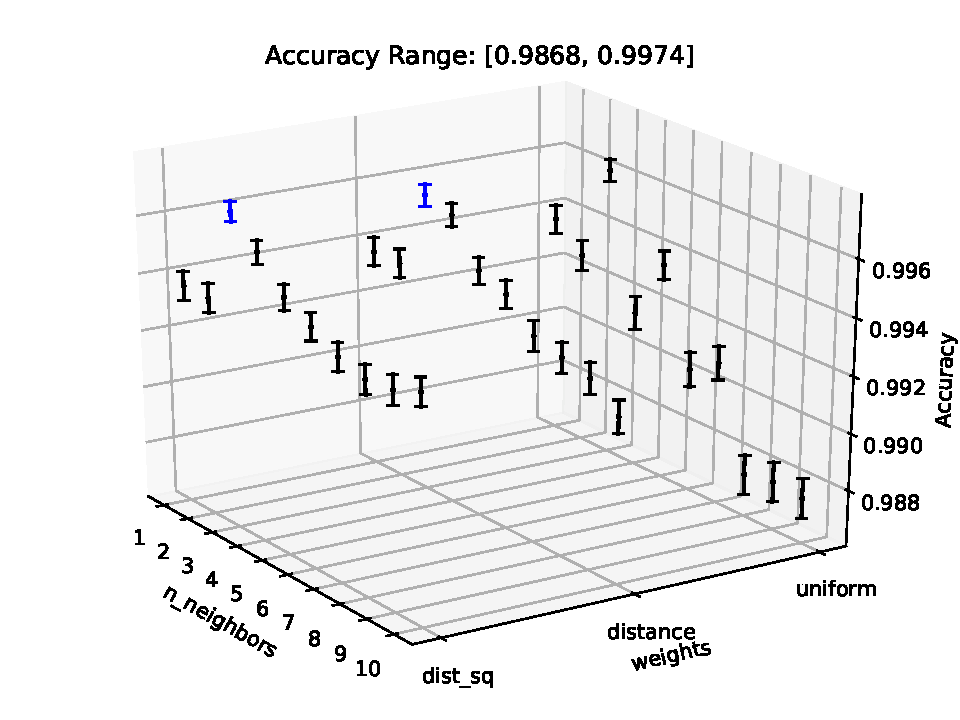
\includegraphics[scale=0.6]{../output/KNN/KNN_941_486/KNN_gridsearch_941_486_global_standard.pdf}
	\caption{Hyper-parameter grid search for $k$ nearest neighbor parameter tuning. The points with the highest (statistically equivalent) accuracies are plotted in blue with all others plotted in black. The grid search was performed using one-hundred times repeated stratified one-hundred-fold cross-validation.}
	\label{fig: knn grid}
\end{figure}

\begin{table}[H]
	\centering
	\caption{Three-fold cross-validation results for tuned $k$ nearest neighbor model.}
	\begin{tabular}{|c|c|c|c|c|c|}
		\hline
		\textbf{Fold} & \textbf{TP} & \textbf{TN} & \textbf{FP} & \textbf{FN} & \textbf{Accuracy} \\ \hline \hline
		1 & 73 & 241 & 0 & 0 & 1.0000  \\ \hline
		2 & 72 & 242 & 0 & 0 & 1.0000  \\ \hline
		3 & 71 & 240 & 1 & 1 & 0.9936  \\ \hline
	\end{tabular}
	\label{tab: cv best knn}
\end{table}

\begin{table}[H]
	\centering
	\caption{Performance results for tuned $k$ nearest neighbor model.}
	\begin{tabular}{|c|c|}
		\hline
		\textbf{Quantity}    & \textbf{Value}       \\ \hline \hline
		Mean Accuracy        & 0.9979 \\ \hline
		Standard Deviation   & 0.0015 \\ \hline
		95.00\% Confidence   & 0.9979 $\pm$ 0.0029 \\ \hline
		Accuracy Range       & (0.9949, 1.0000) \\ \hline
		Best Accuracy        & 1.0000 \\ \hline
		Training Time        & 0.0206 s\\ \hline
		Classification Time  & 0.0235 s \\ \hline
	\end{tabular}
	\label{tab: best knn}
\end{table}

\section{McNemar Tests} \label{sec: mcnemartests}

McNemar's test is a statistical test used on paired data \cite{Raschka}.
It is applied to 2 × 2 contingency tables to determine whether two learning models perform comparably.
Test results comparing all learners are given in Appendix \ref{app: mcnemar}. Since all p-values are not sufficiently small, i.e., less than 0.05, the null hypothesis that two models perform comparably in accuracy cannot be rejected. Thus, the McNemar test shows that all models, including the new neural network and novel ensemble network models, have the same performance.

\section{Conclusions, Future work} \label{sec: conclusion}
The studies in this work focused on three main things: (i) Creating and optimizing a feed-forward neural-network, (ii) Creating and optimizing a novel learner, (iii) Comparing these new learners to the optimized basic learners from previous homework assignments.
\\

The neural network results show that a mini-batch gradient descend with a hyperbolic tangent activation function in the hidden layers yields the shortest training times.
In terms of accuracy, the results indicate that connecting single-input single-output neurons in subsequent layers (one neuron on each layer) decreases the accuracy.
With increasing the number of neurons on the hidden layers, the accuracy goes into saturation where the differences between different models are not statistically significant. 
This occurs because increasing the number of model parameters allows more complex representations of the target function.
However, the test and training times increase with the model parameters, making large neural networks very slow to train.
\\

The novel learner, based on an ensemble of decision trees connected with a small neural network, yields comparable to better accuracy than the neural network. 
This is due to the fact that decision trees are easy to train and for this highly correlated data-set, only shallow trees are obtained.
Since the trees reduce the input to a binary form, a less complex neural net can learn the target function.
This results in a 66\% reduction in training time compared to the neural network.
\\

When compared to the optimized basic learners from previous homework, the McNemar tests show that the probability that these models perform differently is low. 
This indicates that the accuracy of every model is the same statistically.
\\

In general, the introduction of a light correlation filtering to reduce the number of input features in the problem yields a considerable saving in training time while statistically preserving the accuracy of a classifier.
 \\
 
A possible way to extend this work in the future is to further optimize these models with more extensive hyper-parameter spaces and to include a PCA filtering as well.
This work can potentially be improved with the introduction of some background knowledge from the field of computer science.
If the authors had more intricate knowledge of the data and what it represents, they could leverage such knowledge to produce a more comprehensive learning model tailored to the specific problem.


\begin{appendices}
\section{McNemar Test Results} \label{app: mcnemar}

\begin{table}[H]
	\centering
	\caption{McNemar test results for tree and perceptron (p = 5.000e-01)}
	\begin{tabular}{|c||c|c|}
		\hline
		& Tree Correct & Tree Incorrect \\ \hline \hline
		Perceptron Correct & 938 & 2 \\ \hline
		Perceptron Incorrect& 0 & 1 \\ \hline
	\end{tabular}
\end{table}

\begin{table}[H]
	\centering
	\caption{McNemar test results for tree and perceptron forest (p = 1.000e+00)}
	\begin{tabular}{|c||c|c|}
		\hline
		& Tree Correct & Tree Incorrect \\ \hline \hline
		Perceptron Forest Correct & 939 & 1 \\ \hline
		Perceptron Forest Incorrect& 1 & 0 \\ \hline
	\end{tabular}
\end{table}

\begin{table}[H]
	\centering
	\caption{McNemar test results for tree and knn (p = 1.000e+00)}
	\begin{tabular}{|c||c|c|}
		\hline
		& Tree Correct & Tree Incorrect \\ \hline \hline
		Knn Correct & 939 & 1 \\ \hline
		Knn Incorrect& 0 & 1 \\ \hline
	\end{tabular}
\end{table}

\begin{table}[H]
	\centering
	\caption{McNemar test results for tree and neural network (p = 1.250e-01)}
	\begin{tabular}{|c||c|c|}
		\hline
		& Tree Correct & Tree Incorrect \\ \hline \hline
		Neural Network Correct & 936 & 4 \\ \hline
		Neural Network Incorrect& 0 & 1 \\ \hline
	\end{tabular}
\end{table}

\begin{table}[H]
	\centering
	\caption{McNemar test results for tree and ensemble network (p = 6.250e-01)}
	\begin{tabular}{|c||c|c|}
		\hline
		& Tree Correct & Tree Incorrect \\ \hline \hline
		Ensemble Network Correct & 937 & 3 \\ \hline
		Ensemble Network Incorrect& 1 & 0 \\ \hline
	\end{tabular}
\end{table}

\begin{table}[H]
	\centering
	\caption{McNemar test results for perceptron and perceptron forest (p = 6.250e-01)}
	\begin{tabular}{|c||c|c|}
		\hline
		& Perceptron Correct & Perceptron Incorrect \\ \hline \hline
		Perceptron Forest Correct & 937 & 1 \\ \hline
		Perceptron Forest Incorrect& 3 & 0 \\ \hline
	\end{tabular}
\end{table}

\begin{table}[H]
	\centering
	\caption{McNemar test results for perceptron and knn (p = 1.000e+00)}
	\begin{tabular}{|c||c|c|}
		\hline
		& Perceptron Correct & Perceptron Incorrect \\ \hline \hline
		Knn Correct & 938 & 0 \\ \hline
		Knn Incorrect& 1 & 2 \\ \hline
	\end{tabular}
\end{table}

\begin{table}[H]
	\centering
	\caption{McNemar test results for perceptron and neural network (p = 6.250e-01)}
	\begin{tabular}{|c||c|c|}
		\hline
		& Perceptron Correct & Perceptron Incorrect \\ \hline \hline
		Neural Network Correct & 935 & 3 \\ \hline
		Neural Network Incorrect& 1 & 2 \\ \hline
	\end{tabular}
\end{table}

\begin{table}[H]
	\centering
	\caption{McNemar test results for perceptron and ensemble network (p = 1.000e+00)}
	\begin{tabular}{|c||c|c|}
		\hline
		& Perceptron Correct & Perceptron Incorrect \\ \hline \hline
		Ensemble Network Correct & 935 & 3 \\ \hline
		Ensemble Network Incorrect& 3 & 0 \\ \hline
	\end{tabular}
\end{table}

\begin{table}[H]
	\centering
	\caption{McNemar test results for perceptron forest and knn (p = 1.000e+00)}
	\begin{tabular}{|c||c|c|}
		\hline
		& Perceptron Forest Correct & Perceptron Forest Incorrect \\ \hline \hline
		Knn Correct & 938 & 2 \\ \hline
		Knn Incorrect& 1 & 0 \\ \hline
	\end{tabular}
\end{table}

\begin{table}[H]
	\centering
	\caption{McNemar test results for perceptron forest and neural network (p = 2.188e-01)}
	\begin{tabular}{|c||c|c|}
		\hline
		& Perceptron Forest Correct & Perceptron Forest Incorrect \\ \hline \hline
		Neural Network Correct & 935 & 5 \\ \hline
		Neural Network Incorrect& 1 & 0 \\ \hline
	\end{tabular}
\end{table}

\begin{table}[H]
	\centering
	\caption{McNemar test results for perceptron forest and ensemble network (p = 6.250e-01)}
	\begin{tabular}{|c||c|c|}
		\hline
		& Perceptron Forest Correct & Perceptron Forest Incorrect \\ \hline \hline
		Ensemble Network Correct & 937 & 3 \\ \hline
		Ensemble Network Incorrect& 1 & 0 \\ \hline
	\end{tabular}
\end{table}

\begin{table}[H]
	\centering
	\caption{McNemar test results for knn and neural network (p = 2.500e-01)}
	\begin{tabular}{|c||c|c|}
		\hline
		& Knn Correct & Knn Incorrect \\ \hline \hline
		Neural Network Correct & 936 & 3 \\ \hline
		Neural Network Incorrect& 0 & 2 \\ \hline
	\end{tabular}
\end{table}

\begin{table}[H]
	\centering
	\caption{McNemar test results for knn and ensemble network (p = 1.000e+00)}
	\begin{tabular}{|c||c|c|}
		\hline
		& Knn Correct & Knn Incorrect \\ \hline \hline
		Ensemble Network Correct & 936 & 3 \\ \hline
		Ensemble Network Incorrect& 2 & 0 \\ \hline
	\end{tabular}
\end{table}

\begin{table}[H]
	\centering
	\caption{McNemar test results for neural network and ensemble network (p = 6.875e-01)}
	\begin{tabular}{|c||c|c|}
		\hline
		& Neural Network Correct & Neural Network Incorrect \\ \hline \hline
		Ensemble Network Correct & 934 & 2 \\ \hline
		Ensemble Network Incorrect& 4 & 1 \\ \hline
	\end{tabular}
\end{table}
\end{appendices}
\bibliographystyle{ieeetr}
\bibliography{bibliography}


\end{document}
